%!TEX root = ../report.tex
\documentclass[../report.tex]{subfiles}

\begin{document}
    \section{Evaluation}
    \label{sec:evaluation}

    % If your work involved experiments, describe the experimental setup and the results in this section.

    Our experimental evaluation utilized the 'tiny' variant of Whisper\cite{radford2023robust} and the LibriSpeech\cite{panayotov2015librispeech} dataset. We computed influence functions at both the individual token and full sentence levels. Using sampled audio clips from LibriSpeech, we explored multiple parameter combinations: four suppression factors (0.3, 0.5, 0.7, and 0.9) and four window sizes for suppression (3, 5, 7, and 10 frames).
    \begin{figure}[ht]
        \centering
        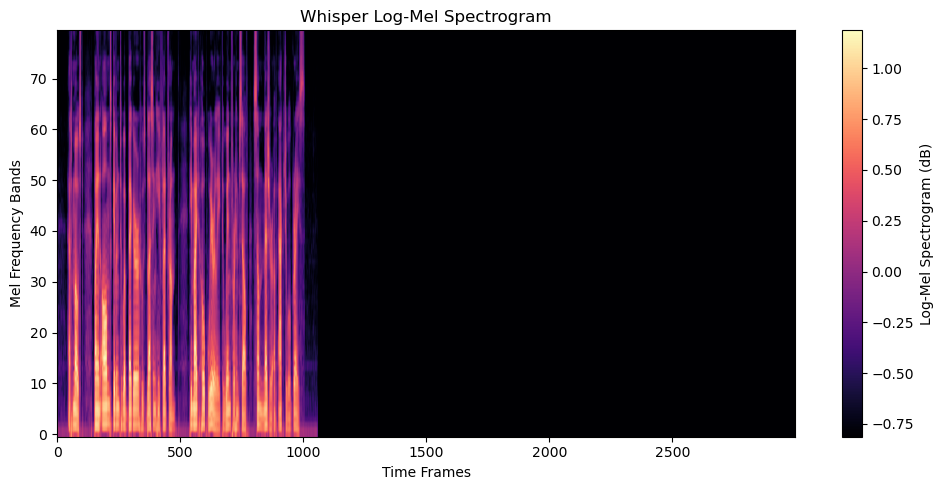
\includegraphics[width=0.48\textwidth]{figures/audio7.png}
        \caption{Log Mel spectrogram of the audio clip for the sentence: \protect\linebreak 
        \textit{At most by an alms given to a beggar whose blessing he fled from he might hope wearily to win for himself some measure of actual grace}}
        \label{fig:mel_spectrogram}
    \end{figure}
    \begin{figure}[ht]
        \centering
        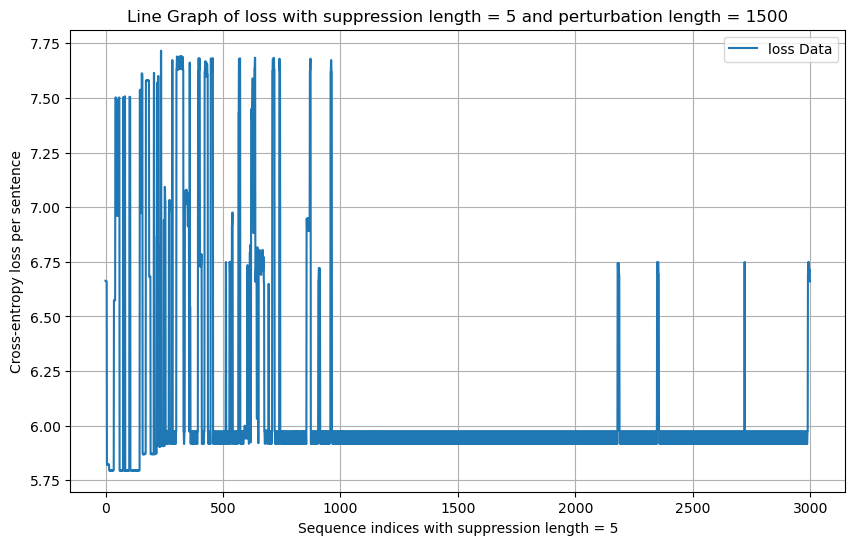
\includegraphics[width=0.5\textwidth]{figures/sentence7_5_5.png}
        \caption{Sentence-level influence map for the transcription of the audio clip in figure \ref{fig:mel_spectrogram}}
        \label{fig:sentence_level_map}
    \end{figure}

    \textbf{Hypothesis 1:} \textit{Frames containing actual speech content show significantly higher influence compared to silent or padded segments of the audio.}

    As shown in figure \ref{fig:sentence_level_map}, we can confirm the hypothesis that frames containing actual speech content show significantly higher influence compared to silent or padded segments of the audio. The other examples also confirm this hypothesis and have been added to the appendix.

    \begin{figure}[p]
        \centering
        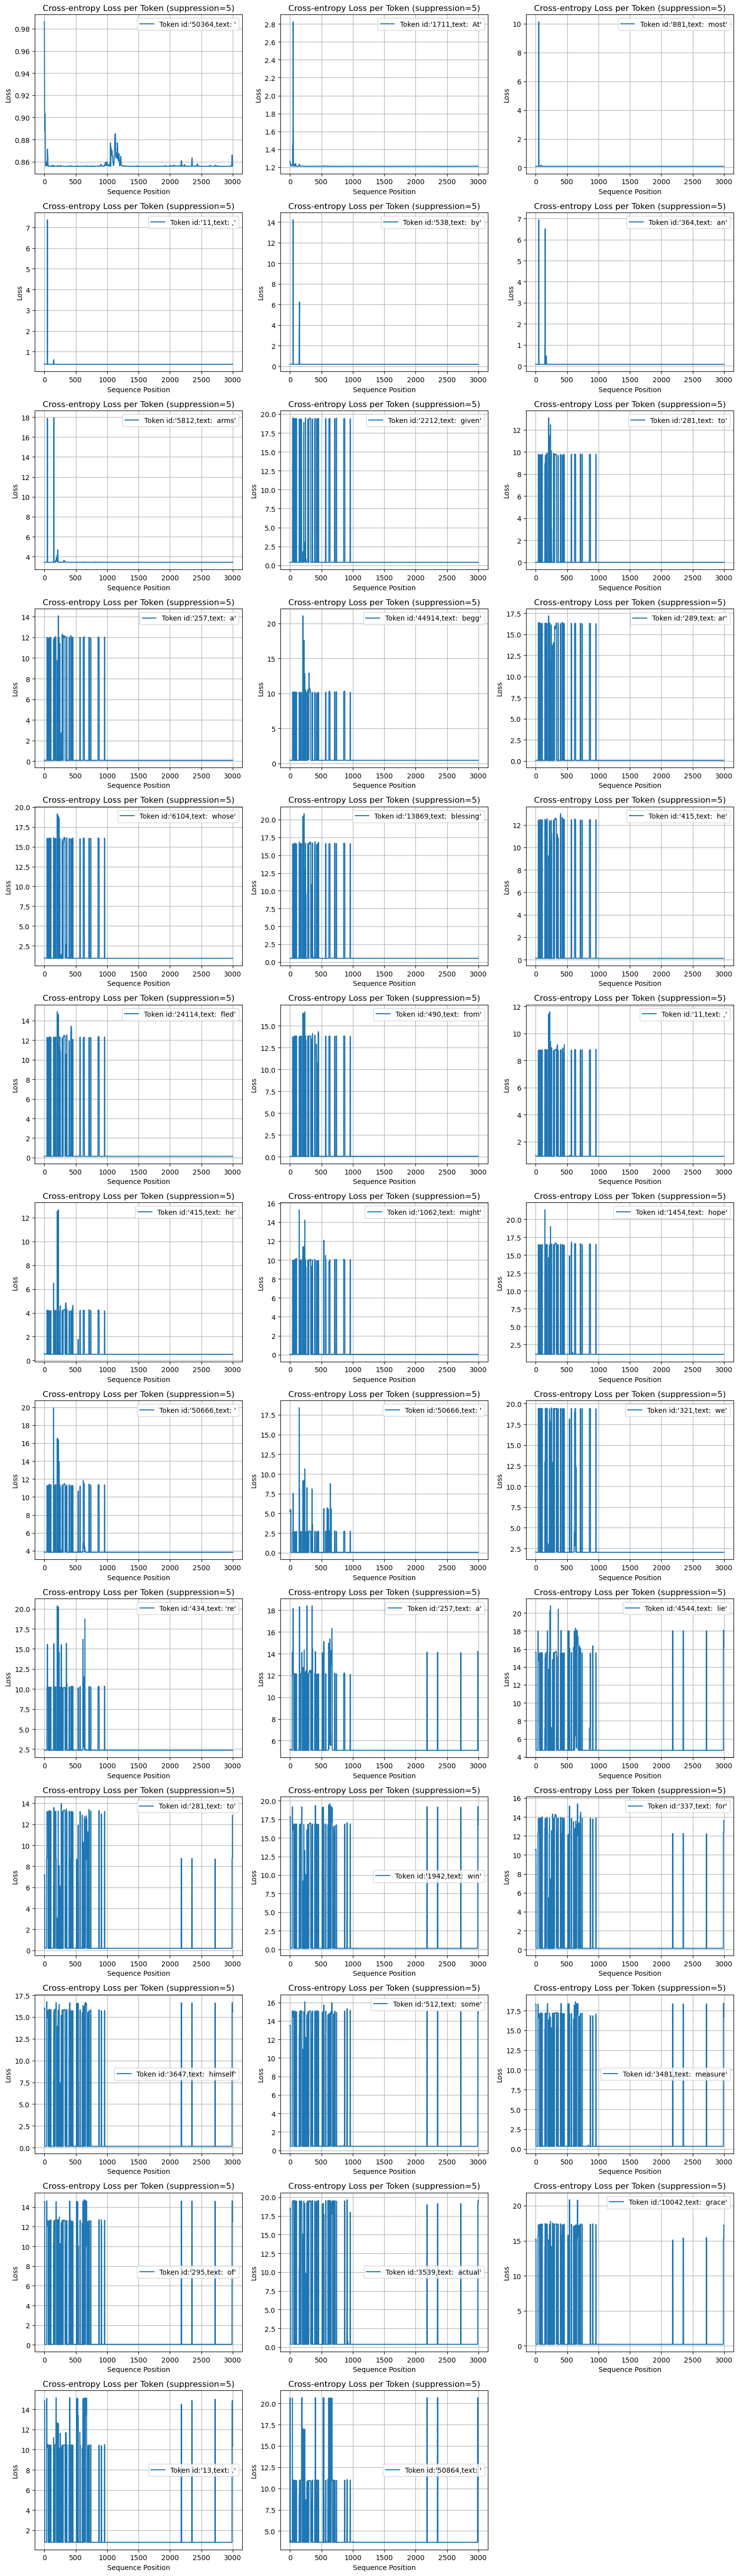
\includegraphics[width=\textwidth,height=0.9\textheight,keepaspectratio]{figures/per_token_5_5.png}
        \caption{Token-level influence maps for the transcription of the audio clip in figure \ref{fig:mel_spectrogram}}
        \label{fig:token_level_map}
    \end{figure}

    \textbf{Hypothesis 2:} \textit{The temporal frames immediately preceding a token has the strongest influence on the model's prediction of that token.}

    Analysis of figure \ref{fig:token_level_map} reveals that the model's token predictions were most heavily influenced by the temporal frames that directly preceded each token. Additionally, we observed that for tokens located near padded regions, the padded temporal frames also exhibited influence on the model's predictions.

    \begin{figure}[ht]
        \centering
        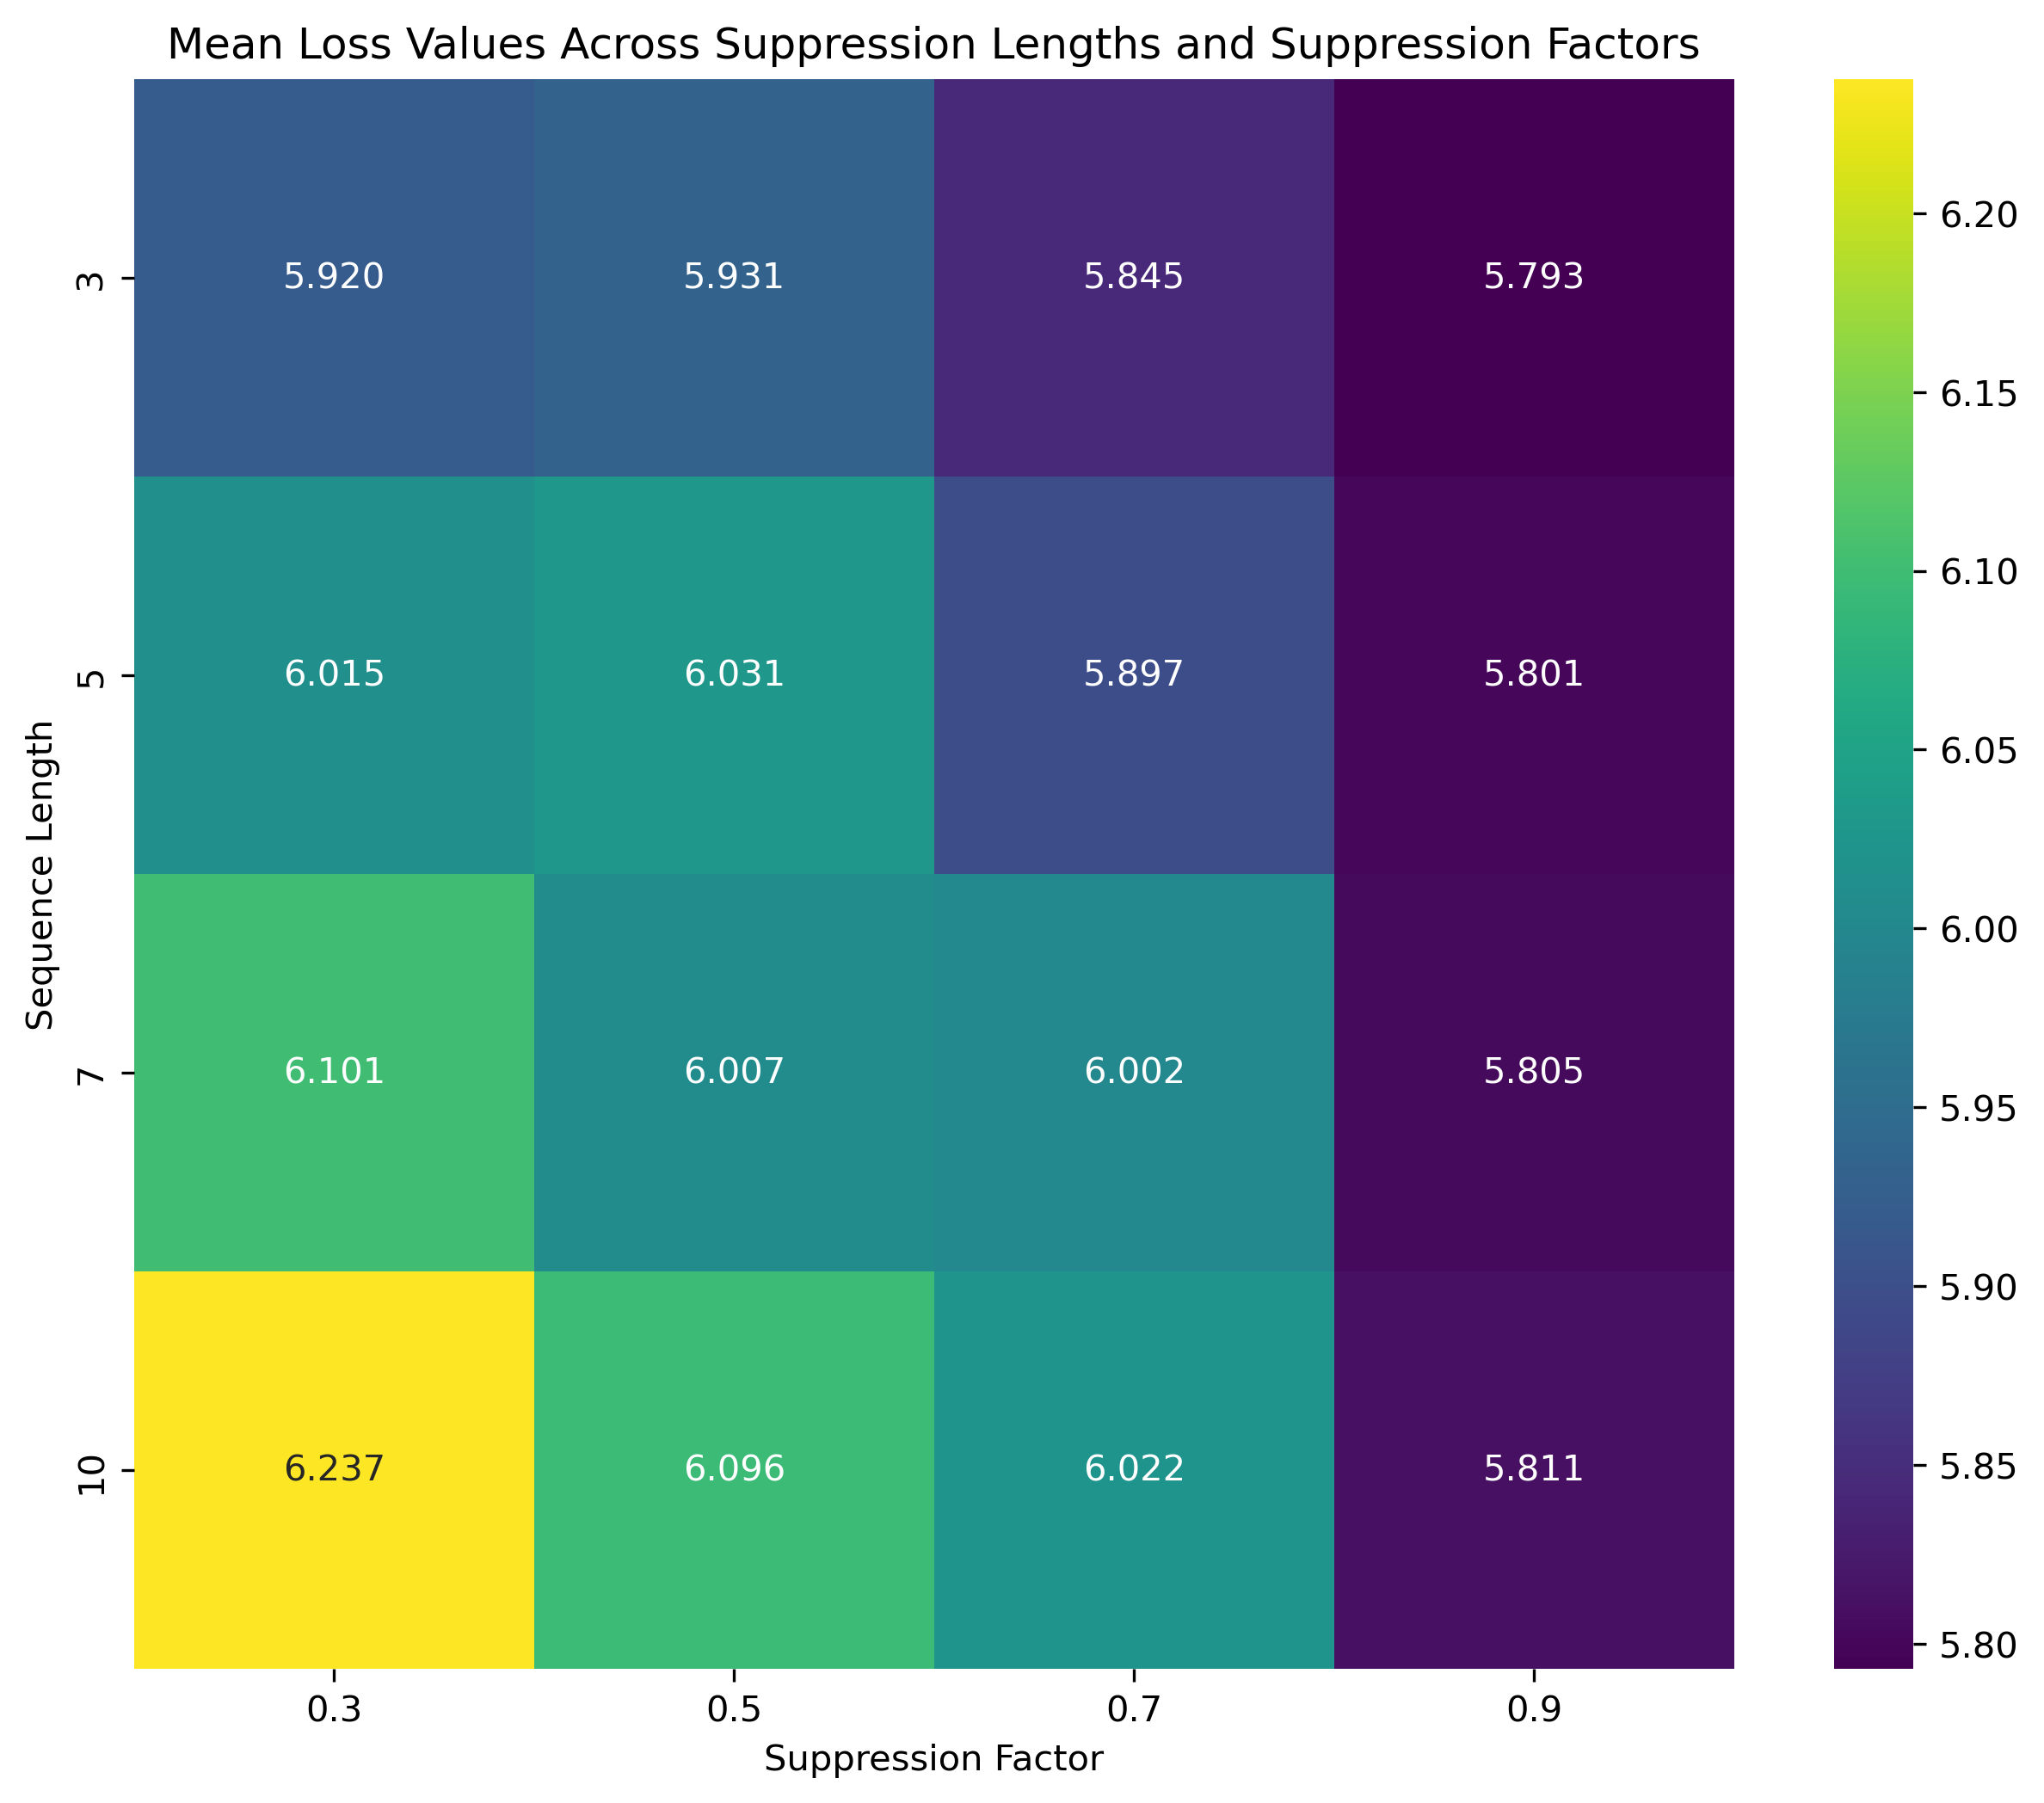
\includegraphics[width=0.5\textwidth]{figures/mean_loss_heatmap.png}
        \caption{Heatmap for the audio clip in figure \ref{fig:mel_spectrogram} showing the mean cross entropy loss for sentence across different suppression factors and window sizes}
        \label{fig:mean_loss_heatmap}
    \end{figure}

    \textbf{Hypothesis 3:} \textit{Larger suppression windows and more aggressive suppression factors (values closer to zero) result in greater disruption to the model's predictions.}

    Figure \ref{fig:mean_loss_heatmap} demonstrates that both increasing the suppression window size and using more aggressive suppression factors leads to greater disruption in model predictions. This is evident from two key observations: First, when more temporal frames are suppressed through larger window sizes, the cross-entropy loss increases substantially. Second, suppression factors closer to zero apply stronger suppression to the frames, effectively diminishing their contribution to the model's attention mechanism and resulting in higher prediction errors.

    \begin{figure}[p]
        \centering
        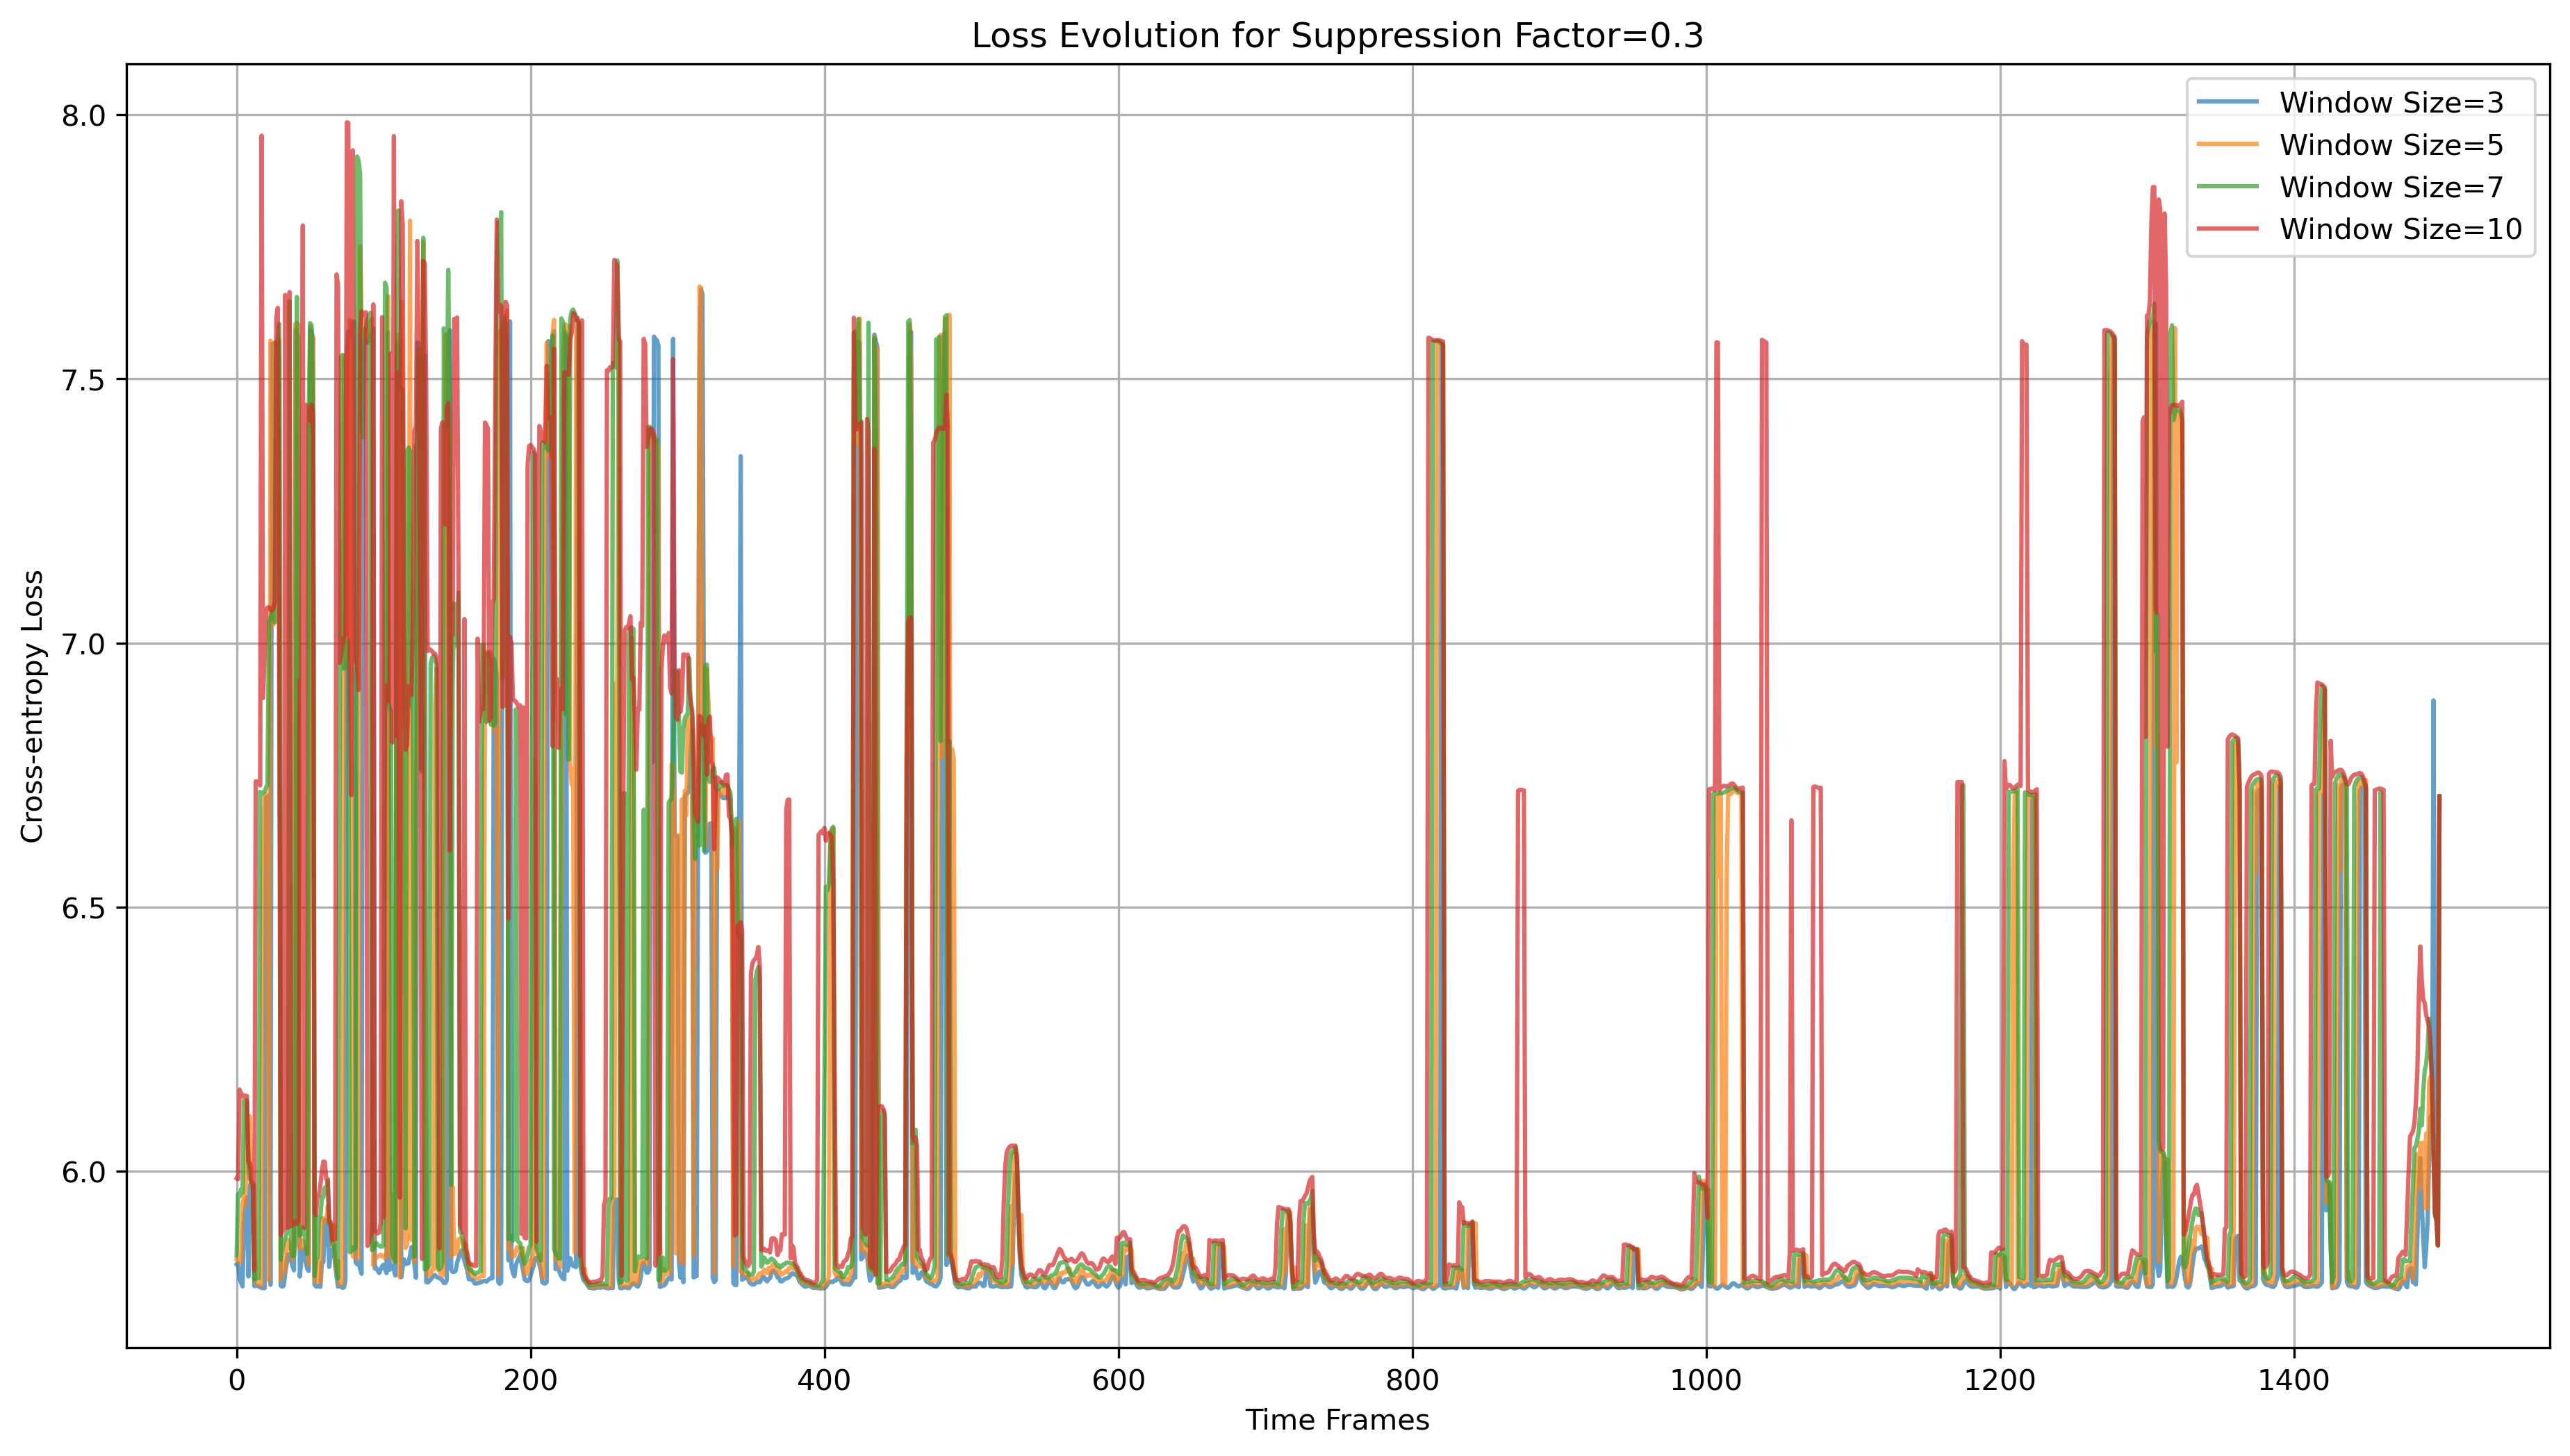
\includegraphics[width=0.48\textwidth]{figures/factor_0.3_comparison.png}
        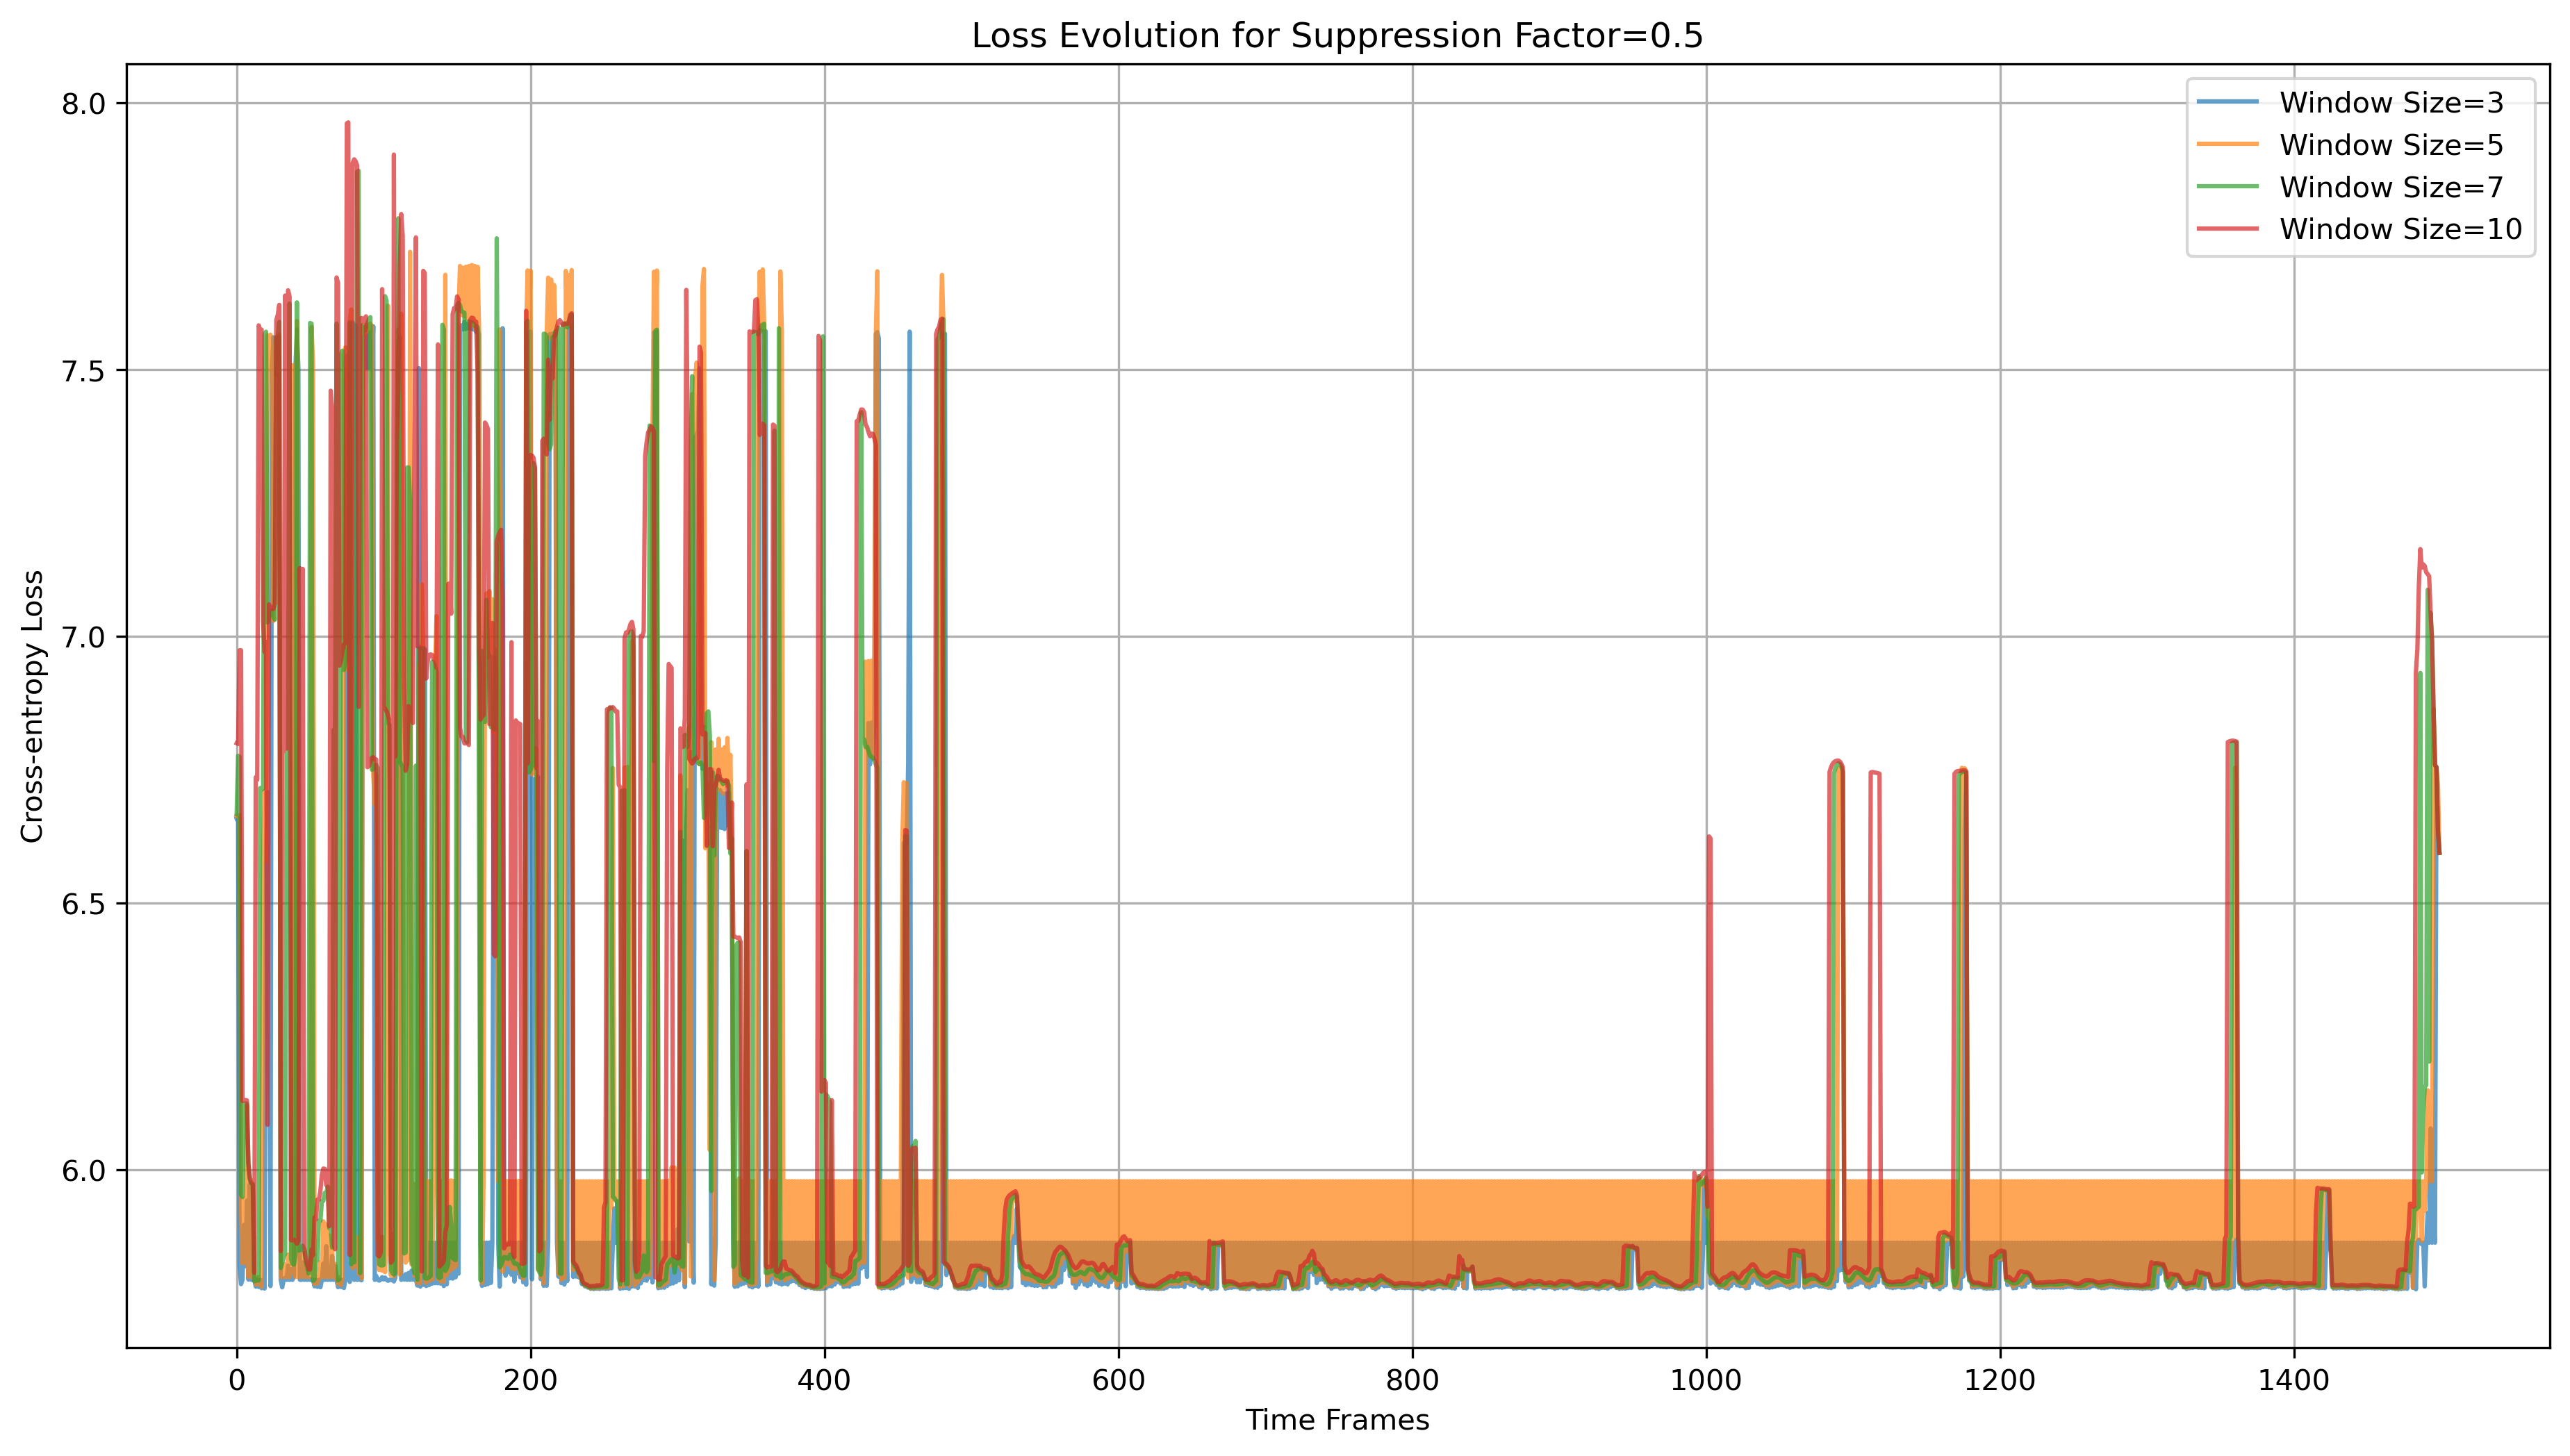
\includegraphics[width=0.48\textwidth]{figures/factor_0.5_comparison.png}
        
        \vspace{1em}
        
        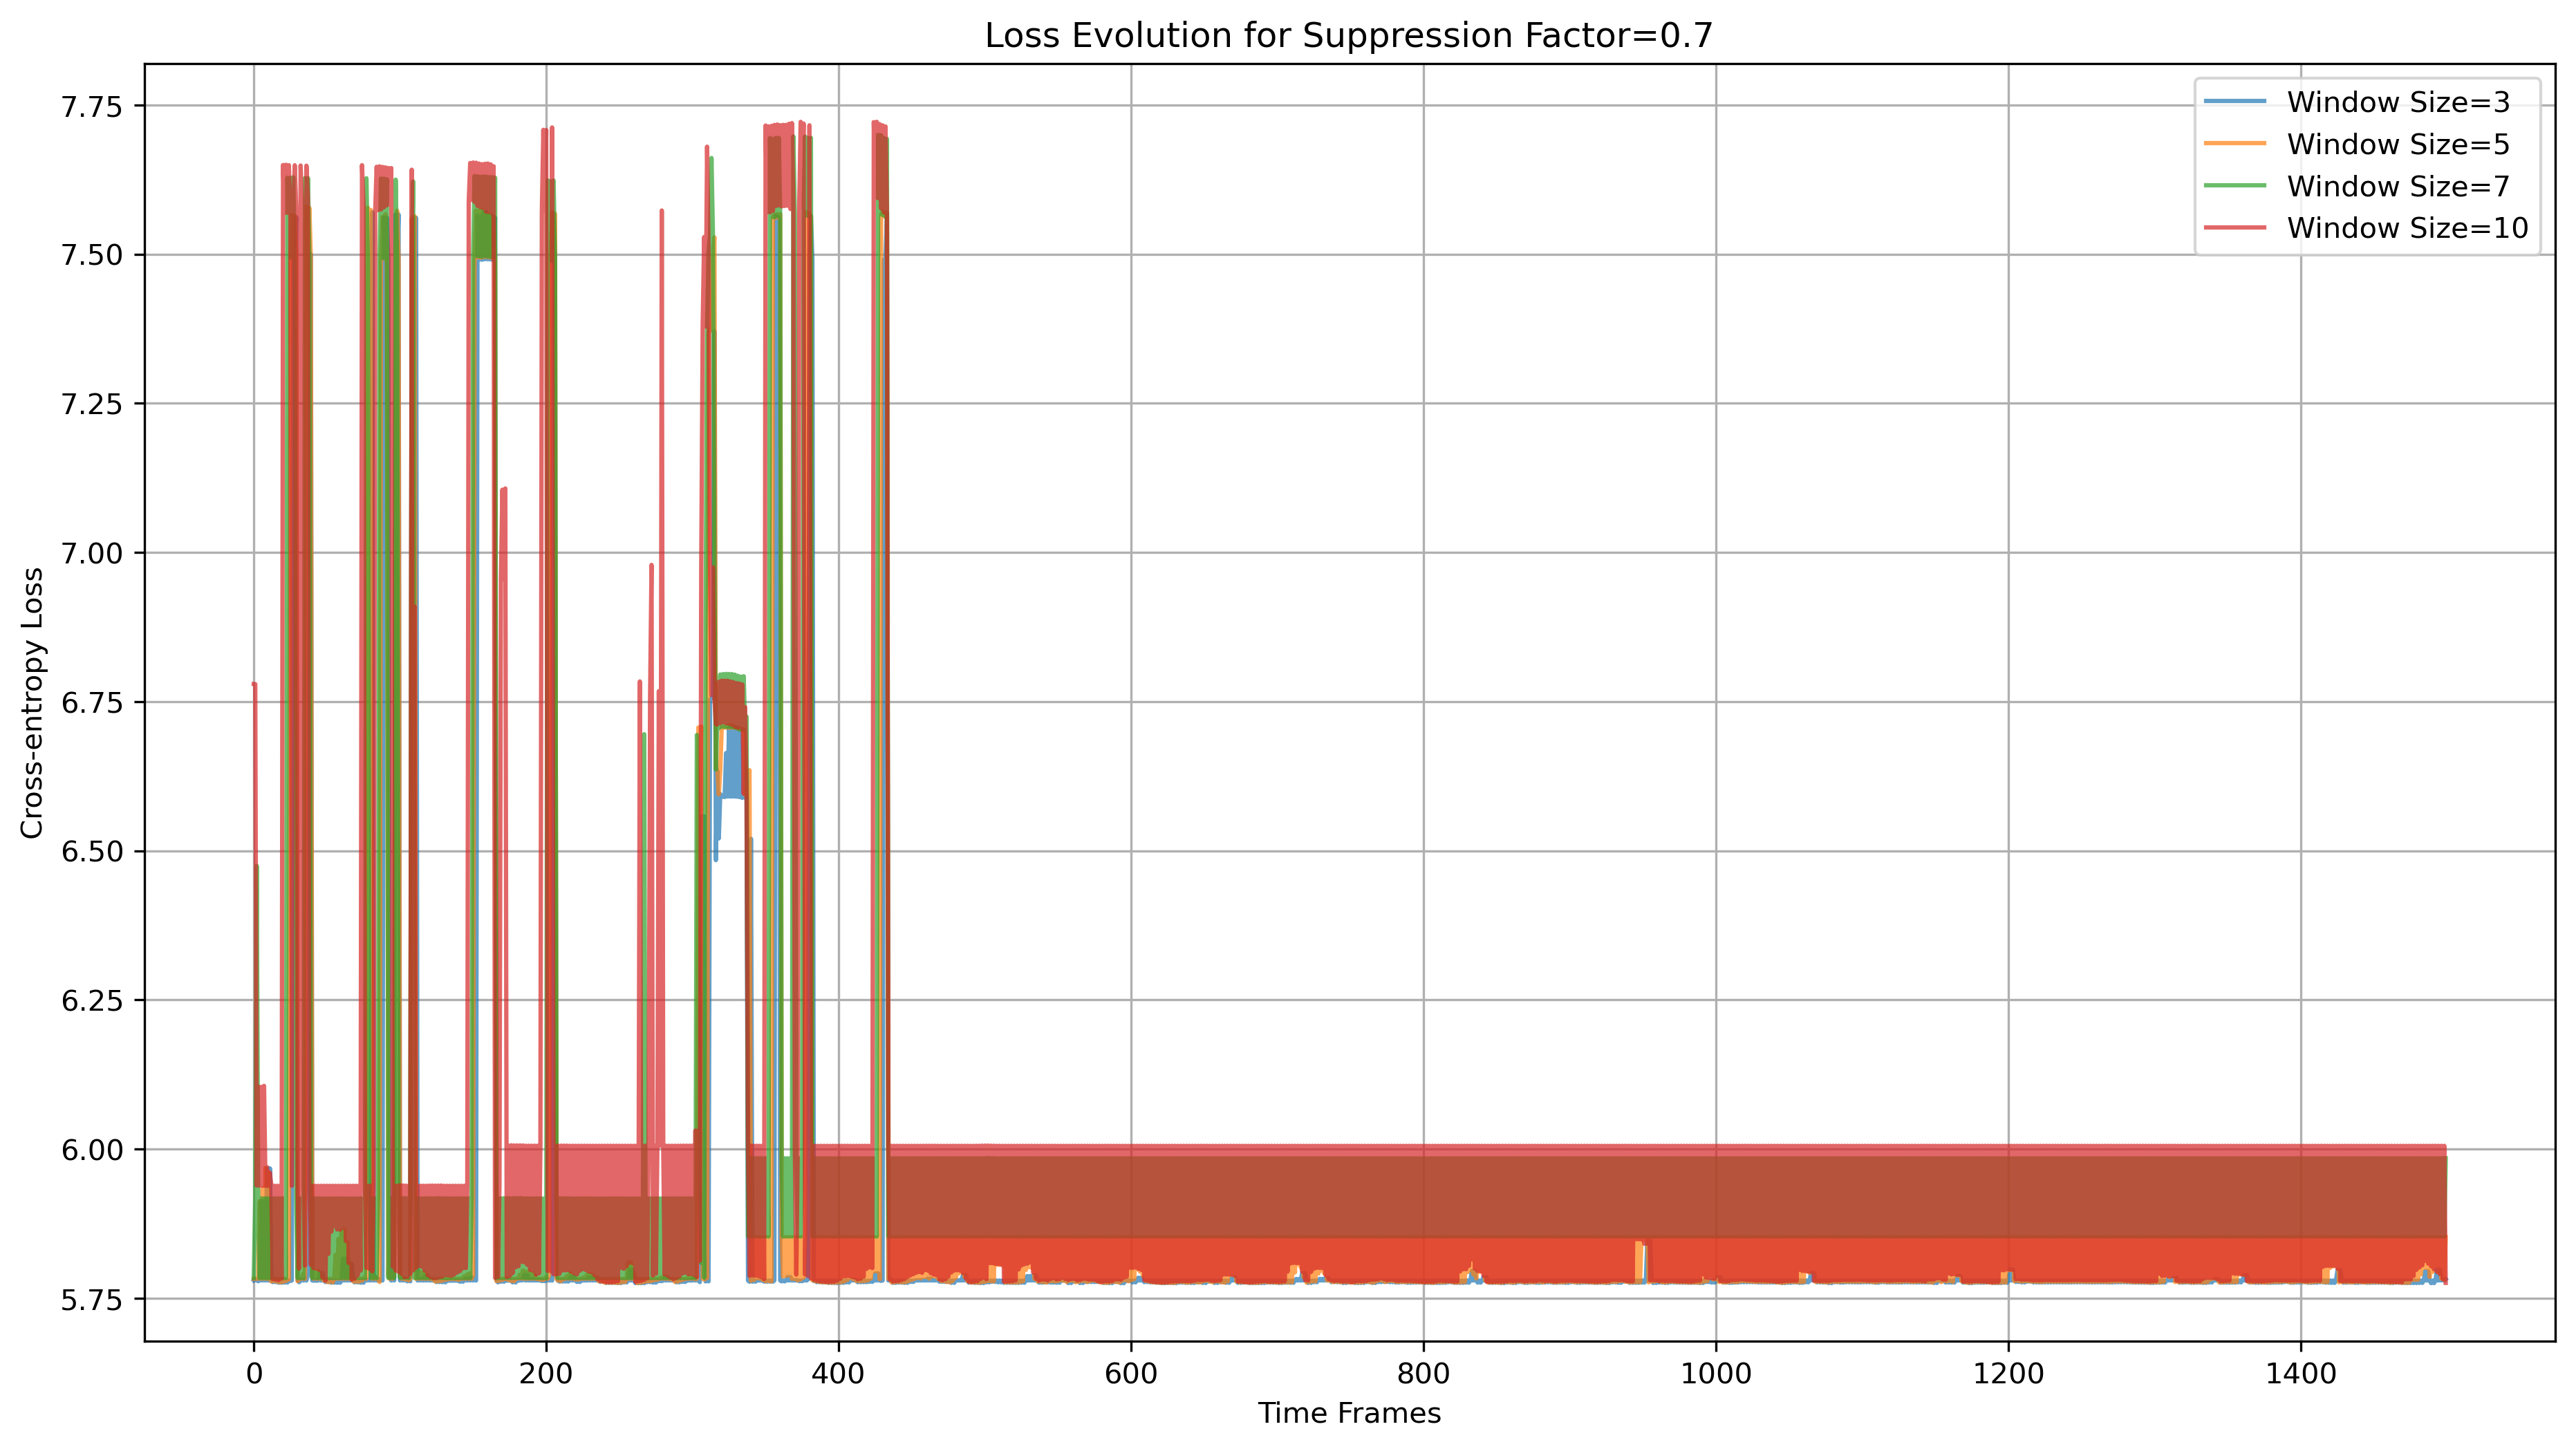
\includegraphics[width=0.48\textwidth]{figures/factor_0.7_comparison.png}
        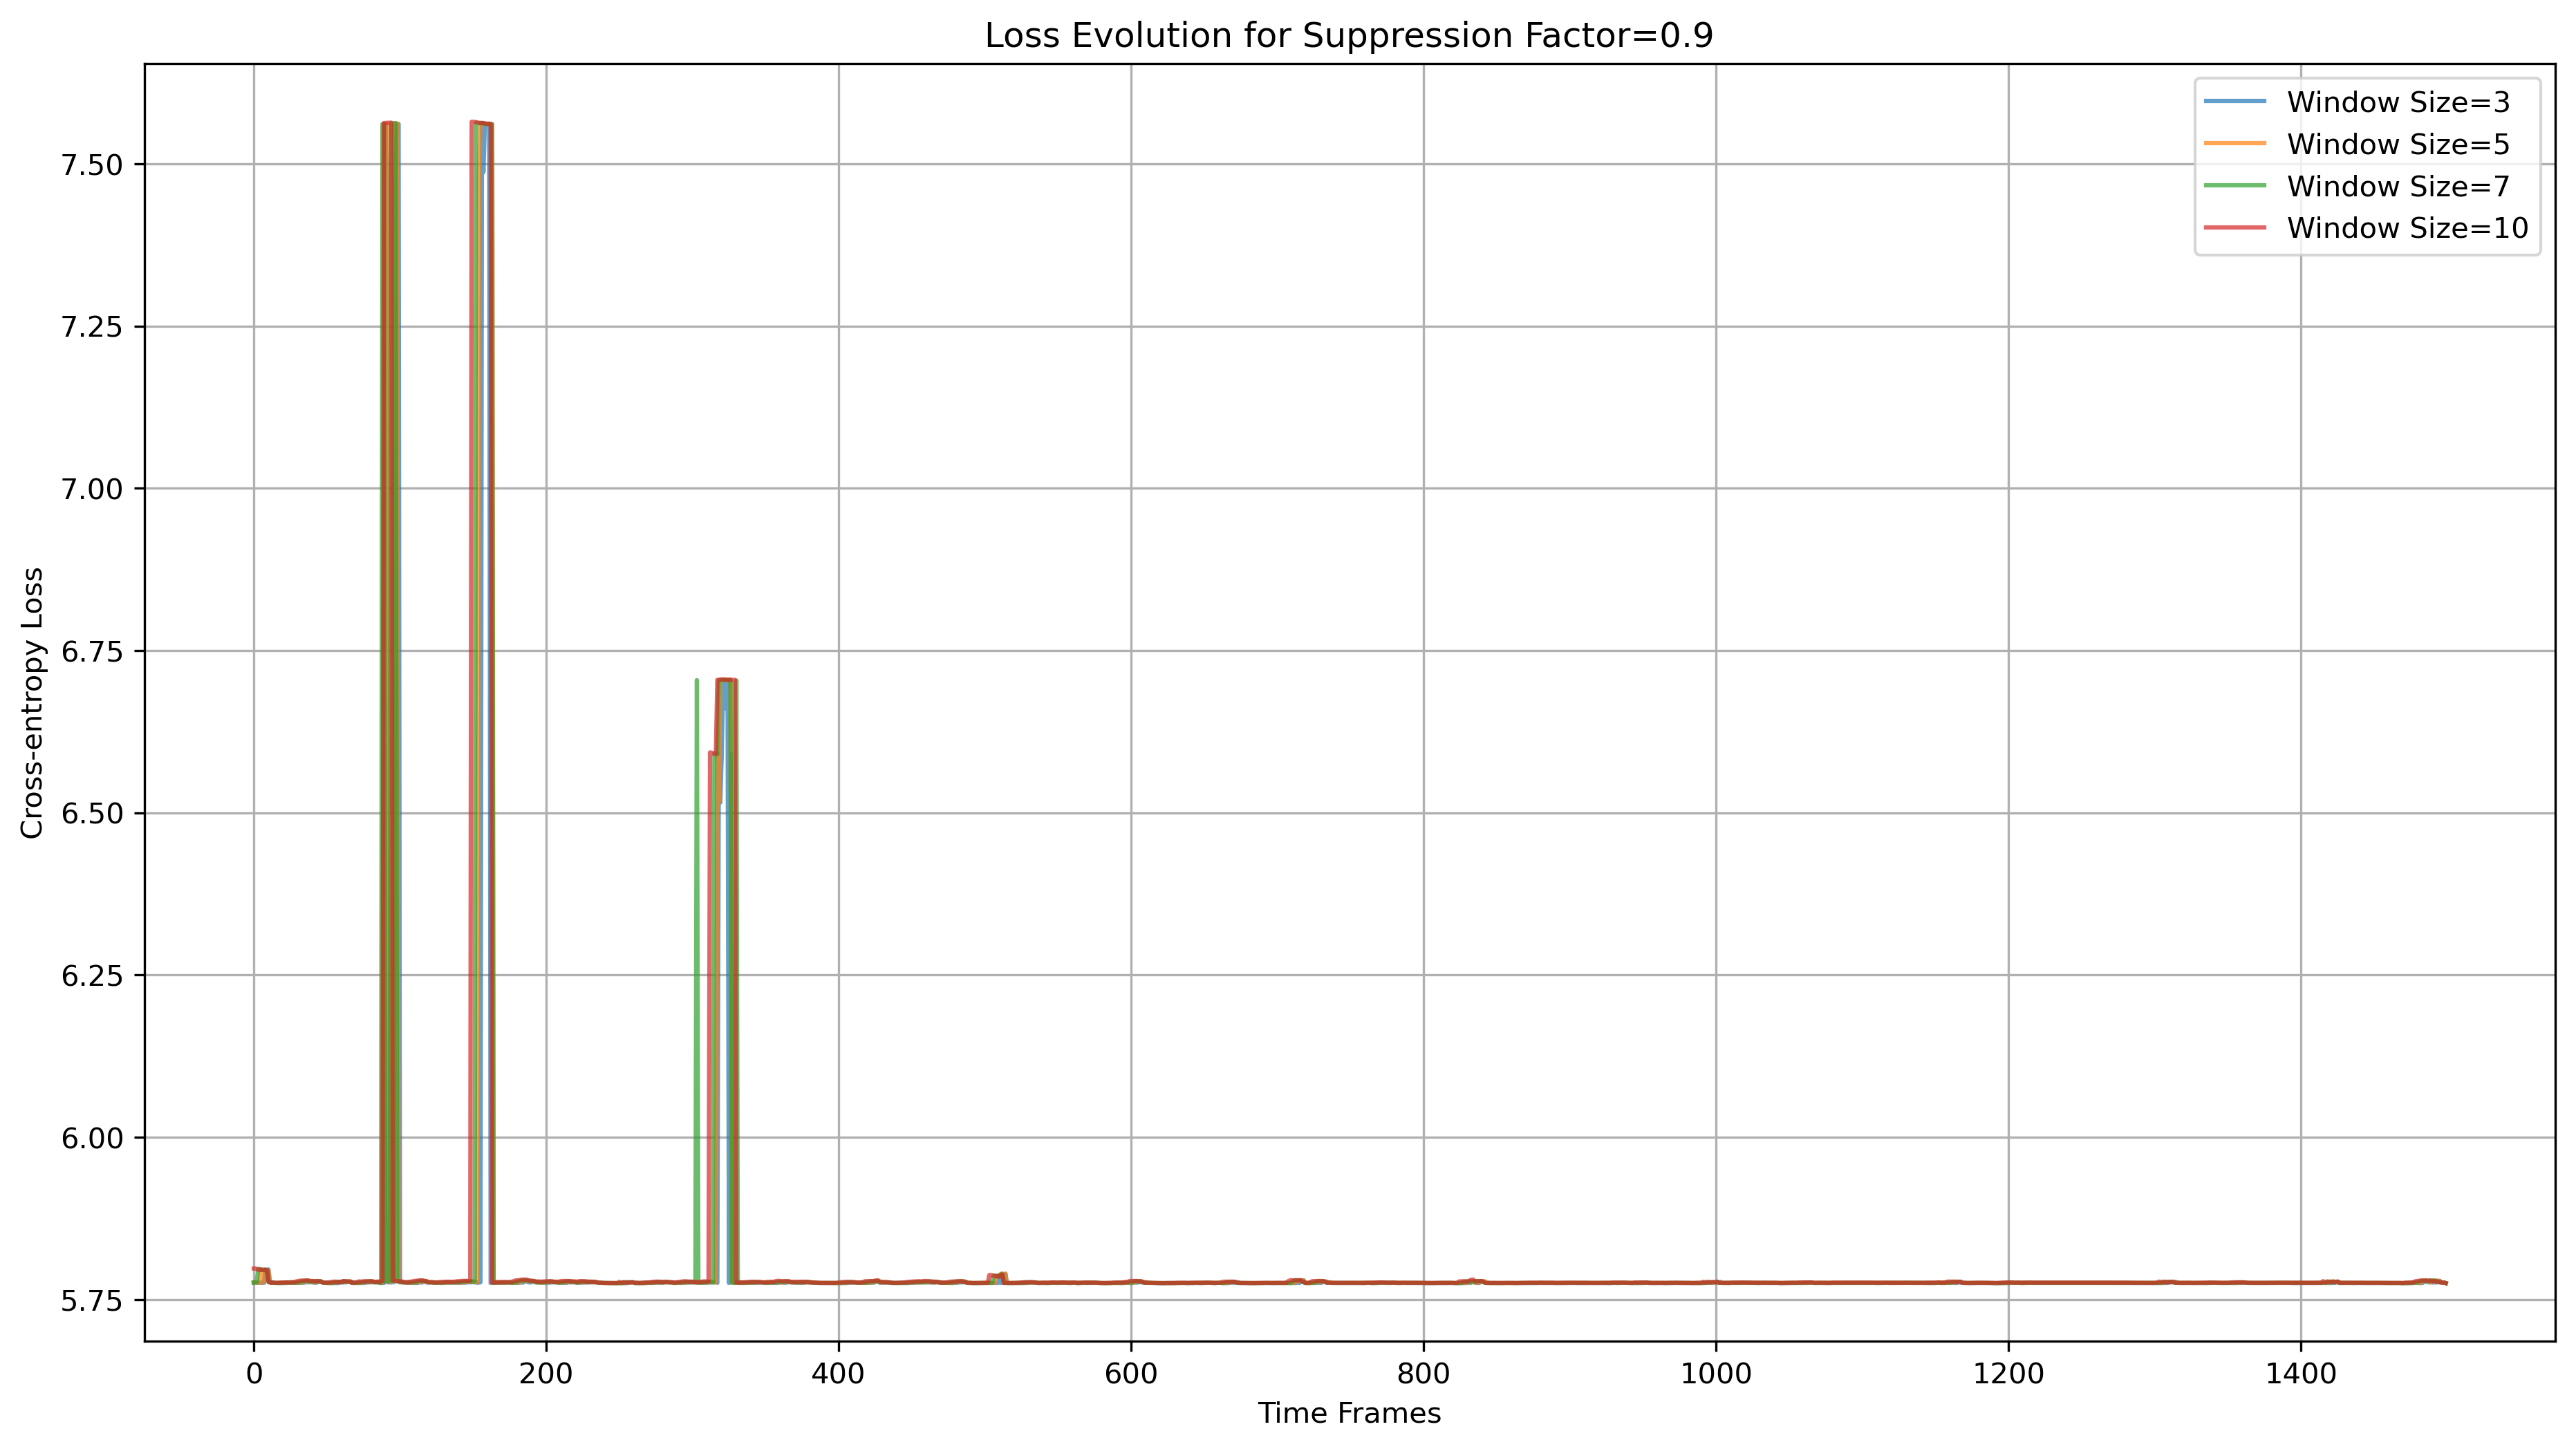
\includegraphics[width=0.48\textwidth]{figures/factor_0.9_comparison.png}
        
        \caption{Cross entropy loss for a suppression factor across different window sizes  over time frames}
        \label{fig:window_comparison}
    \end{figure}

    
    In figure \ref{fig:window_comparison} and \ref{fig:sequence_plots}, we can analyze that even with lower suppression factors like 0.9, the cross entropy loss for larger window sizes is comparable to that of small window sizes for same suppression factor. Even with increased window size it did not impact the loss evolution much.
    
   

    \begin{figure}[p]
        \centering
        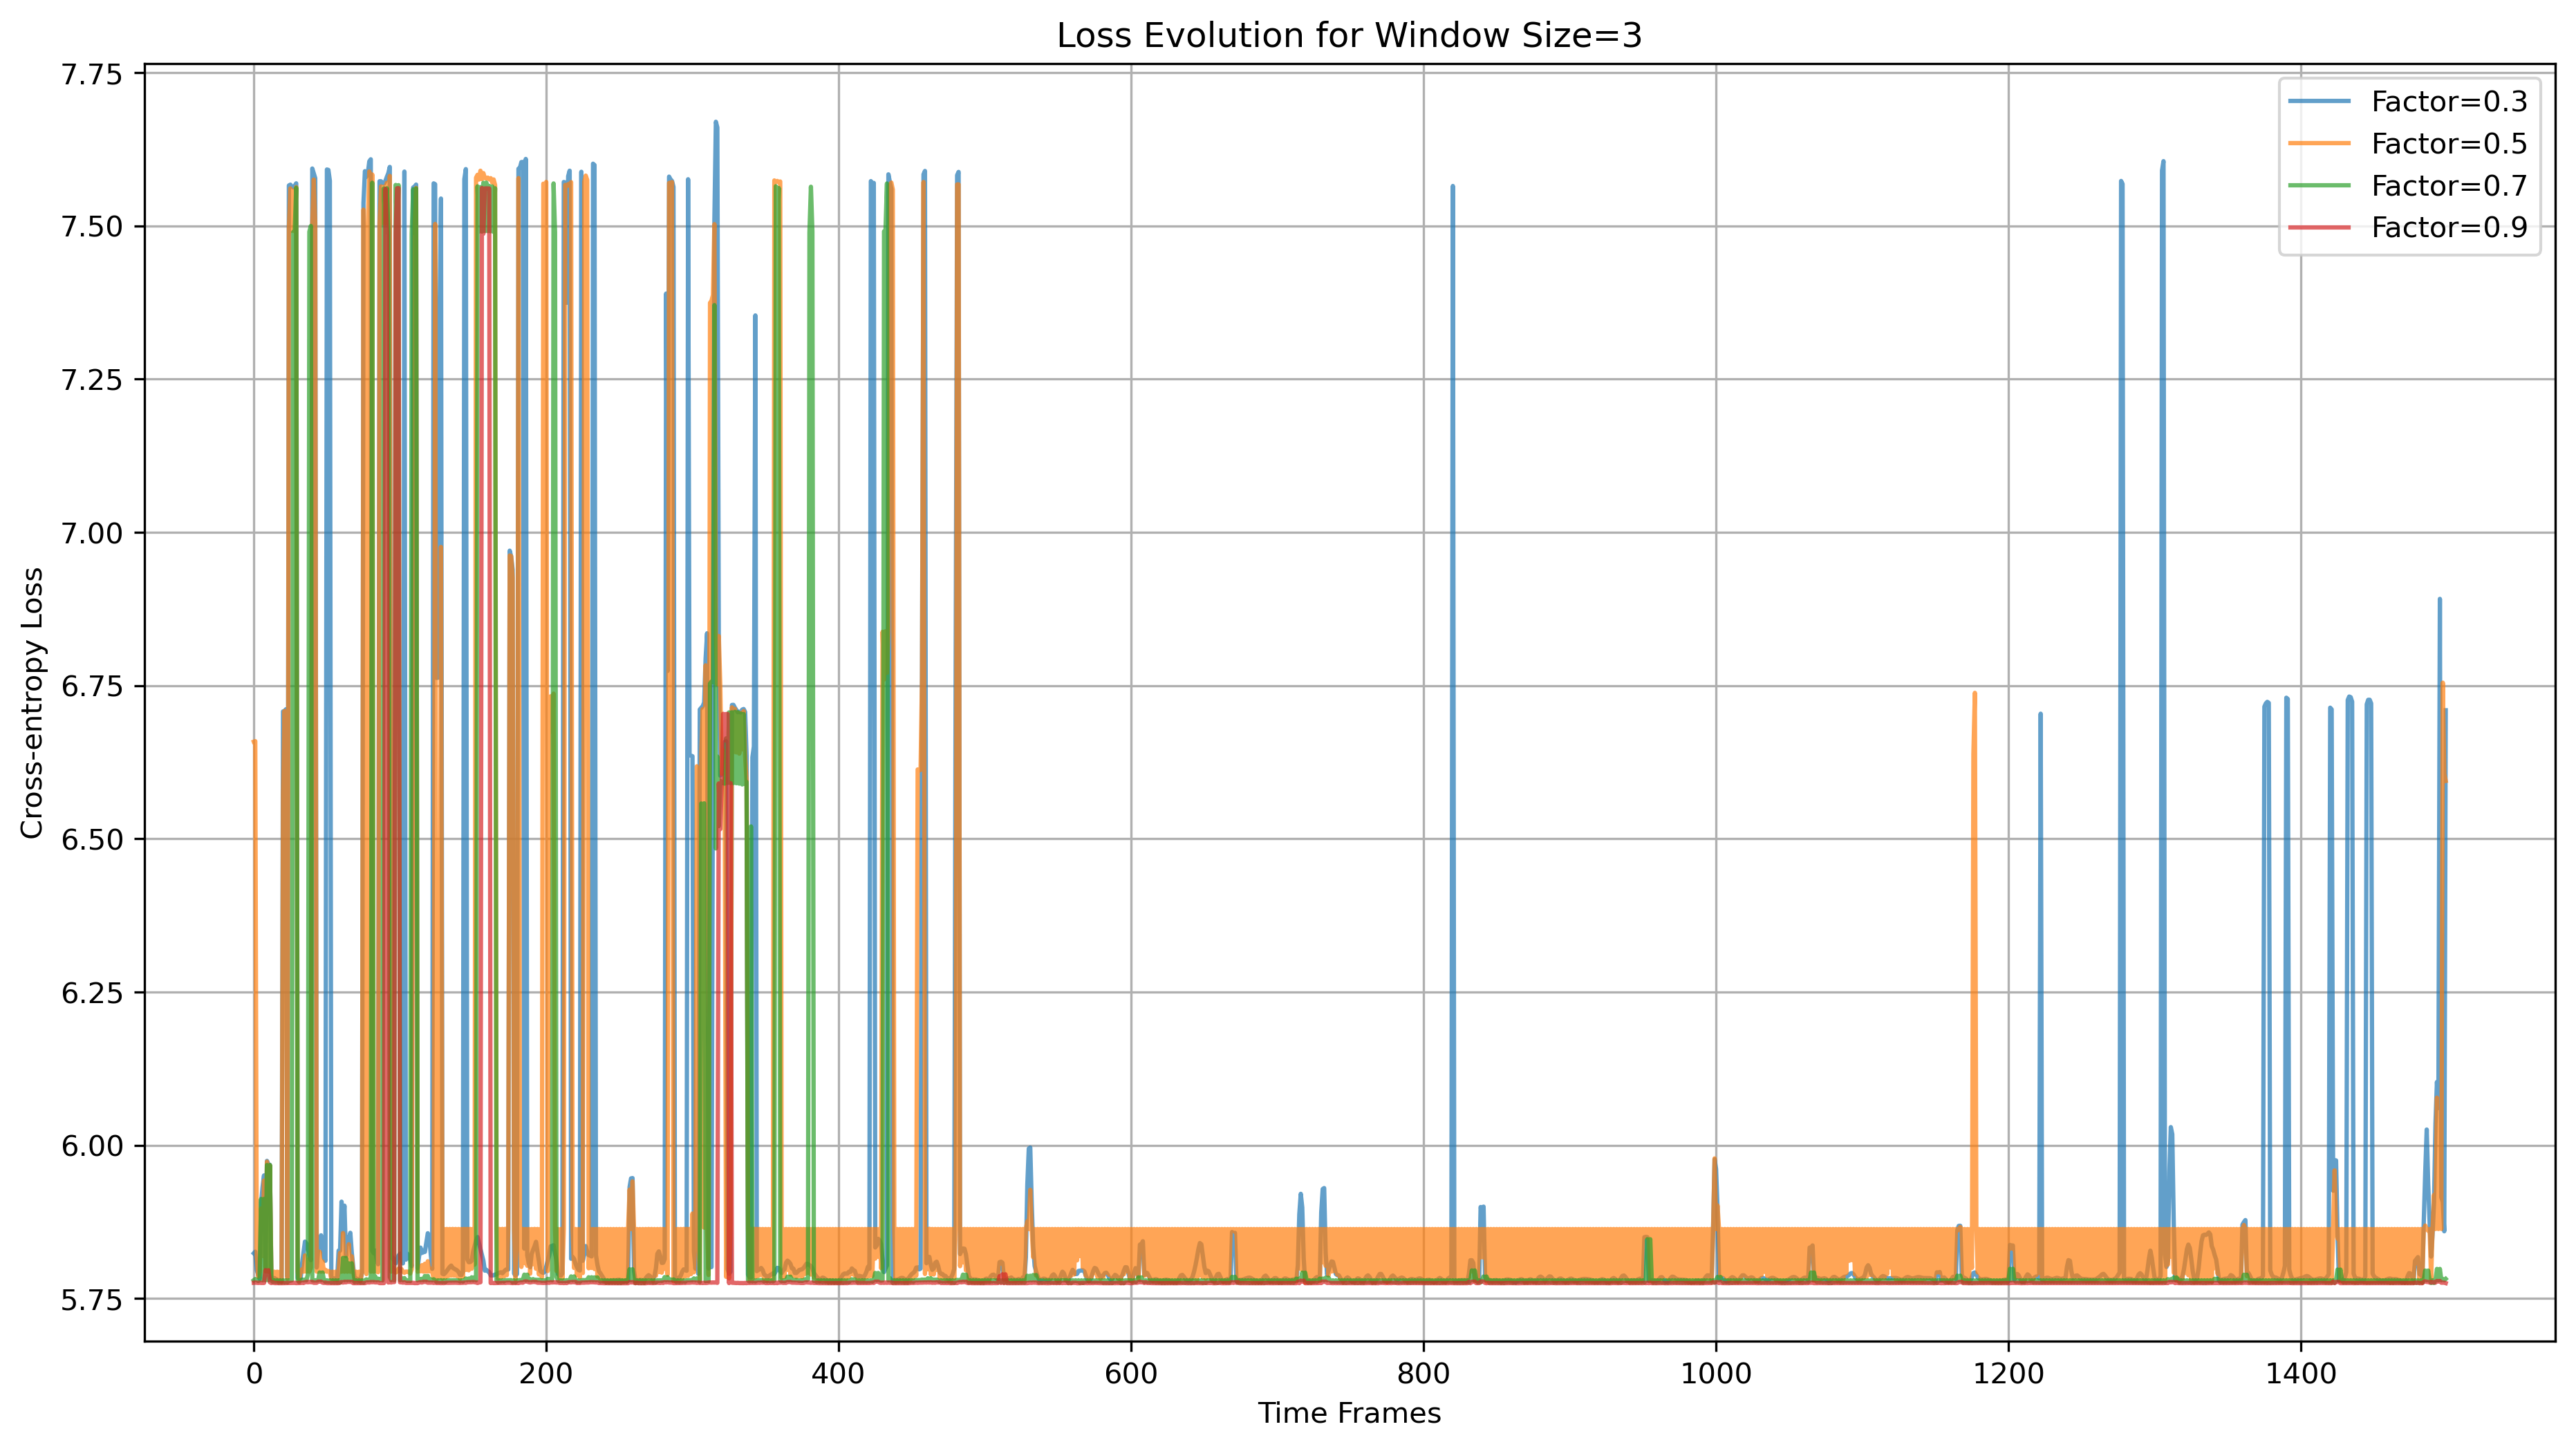
\includegraphics[width=0.48\textwidth]{figures/seq_len_3_comparison.png}
        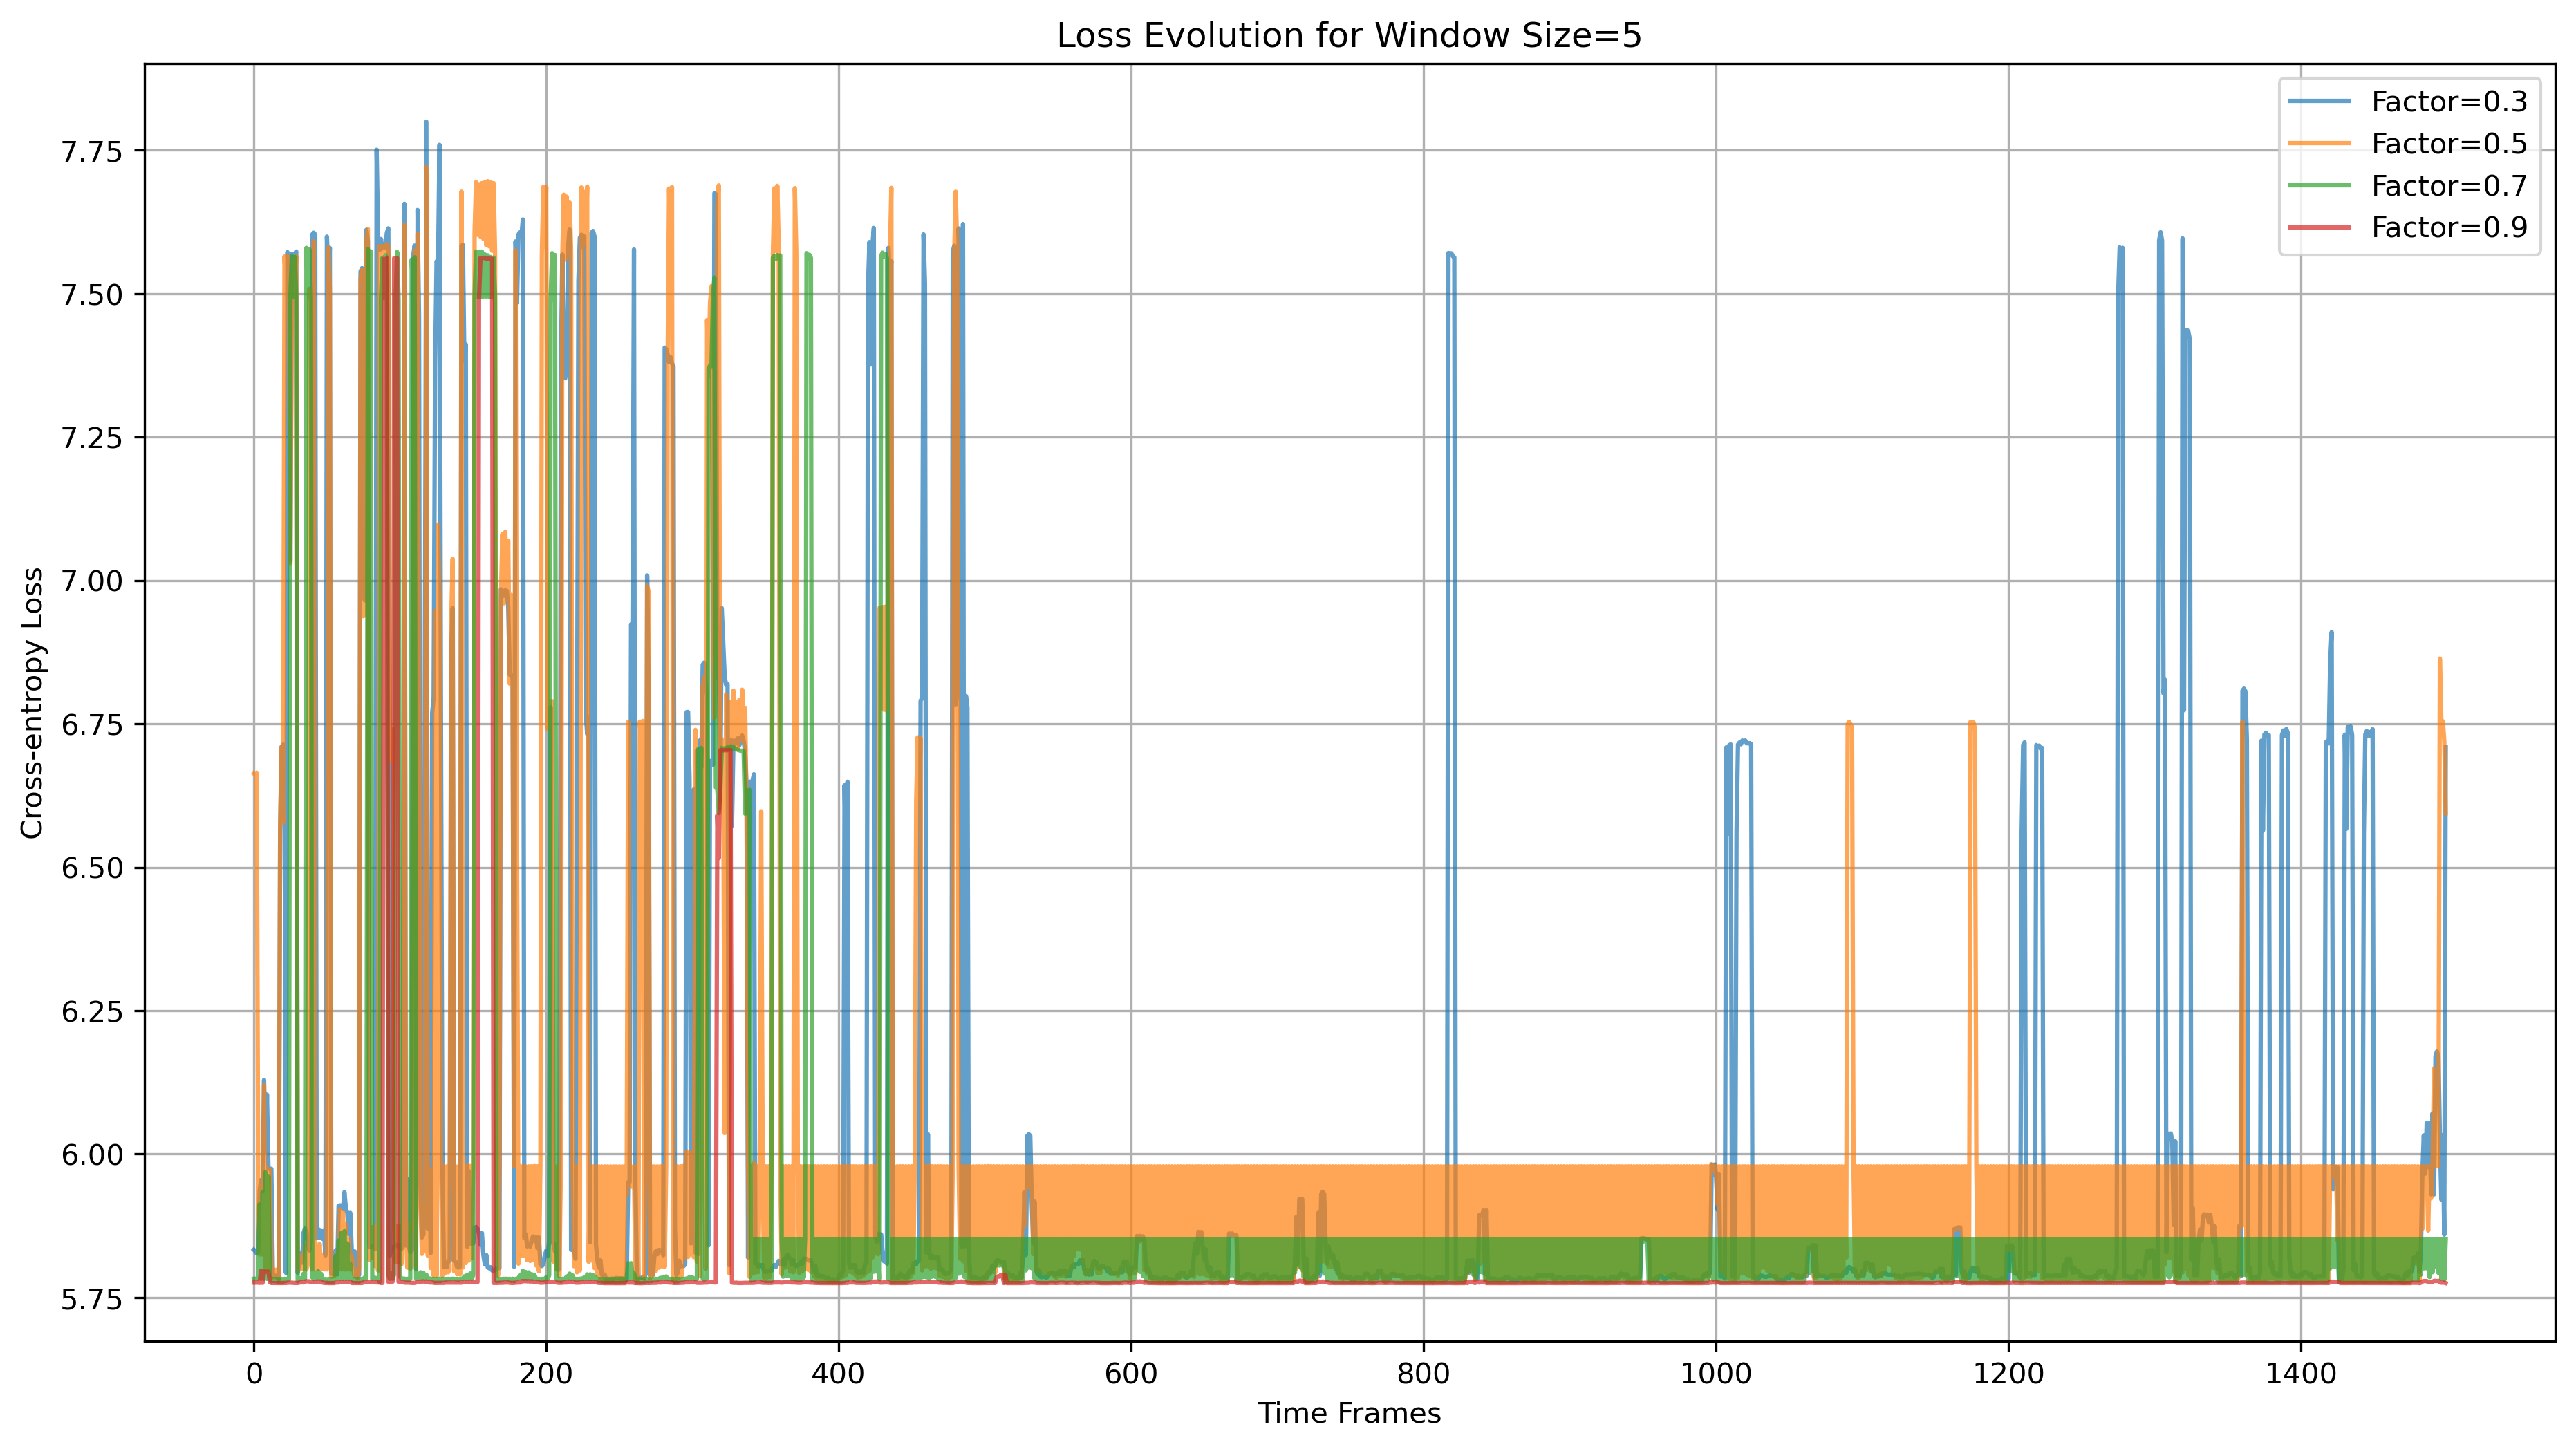
\includegraphics[width=0.48\textwidth]{figures/seq_len_5_comparison.png}
        
        \vspace{1em}
        
        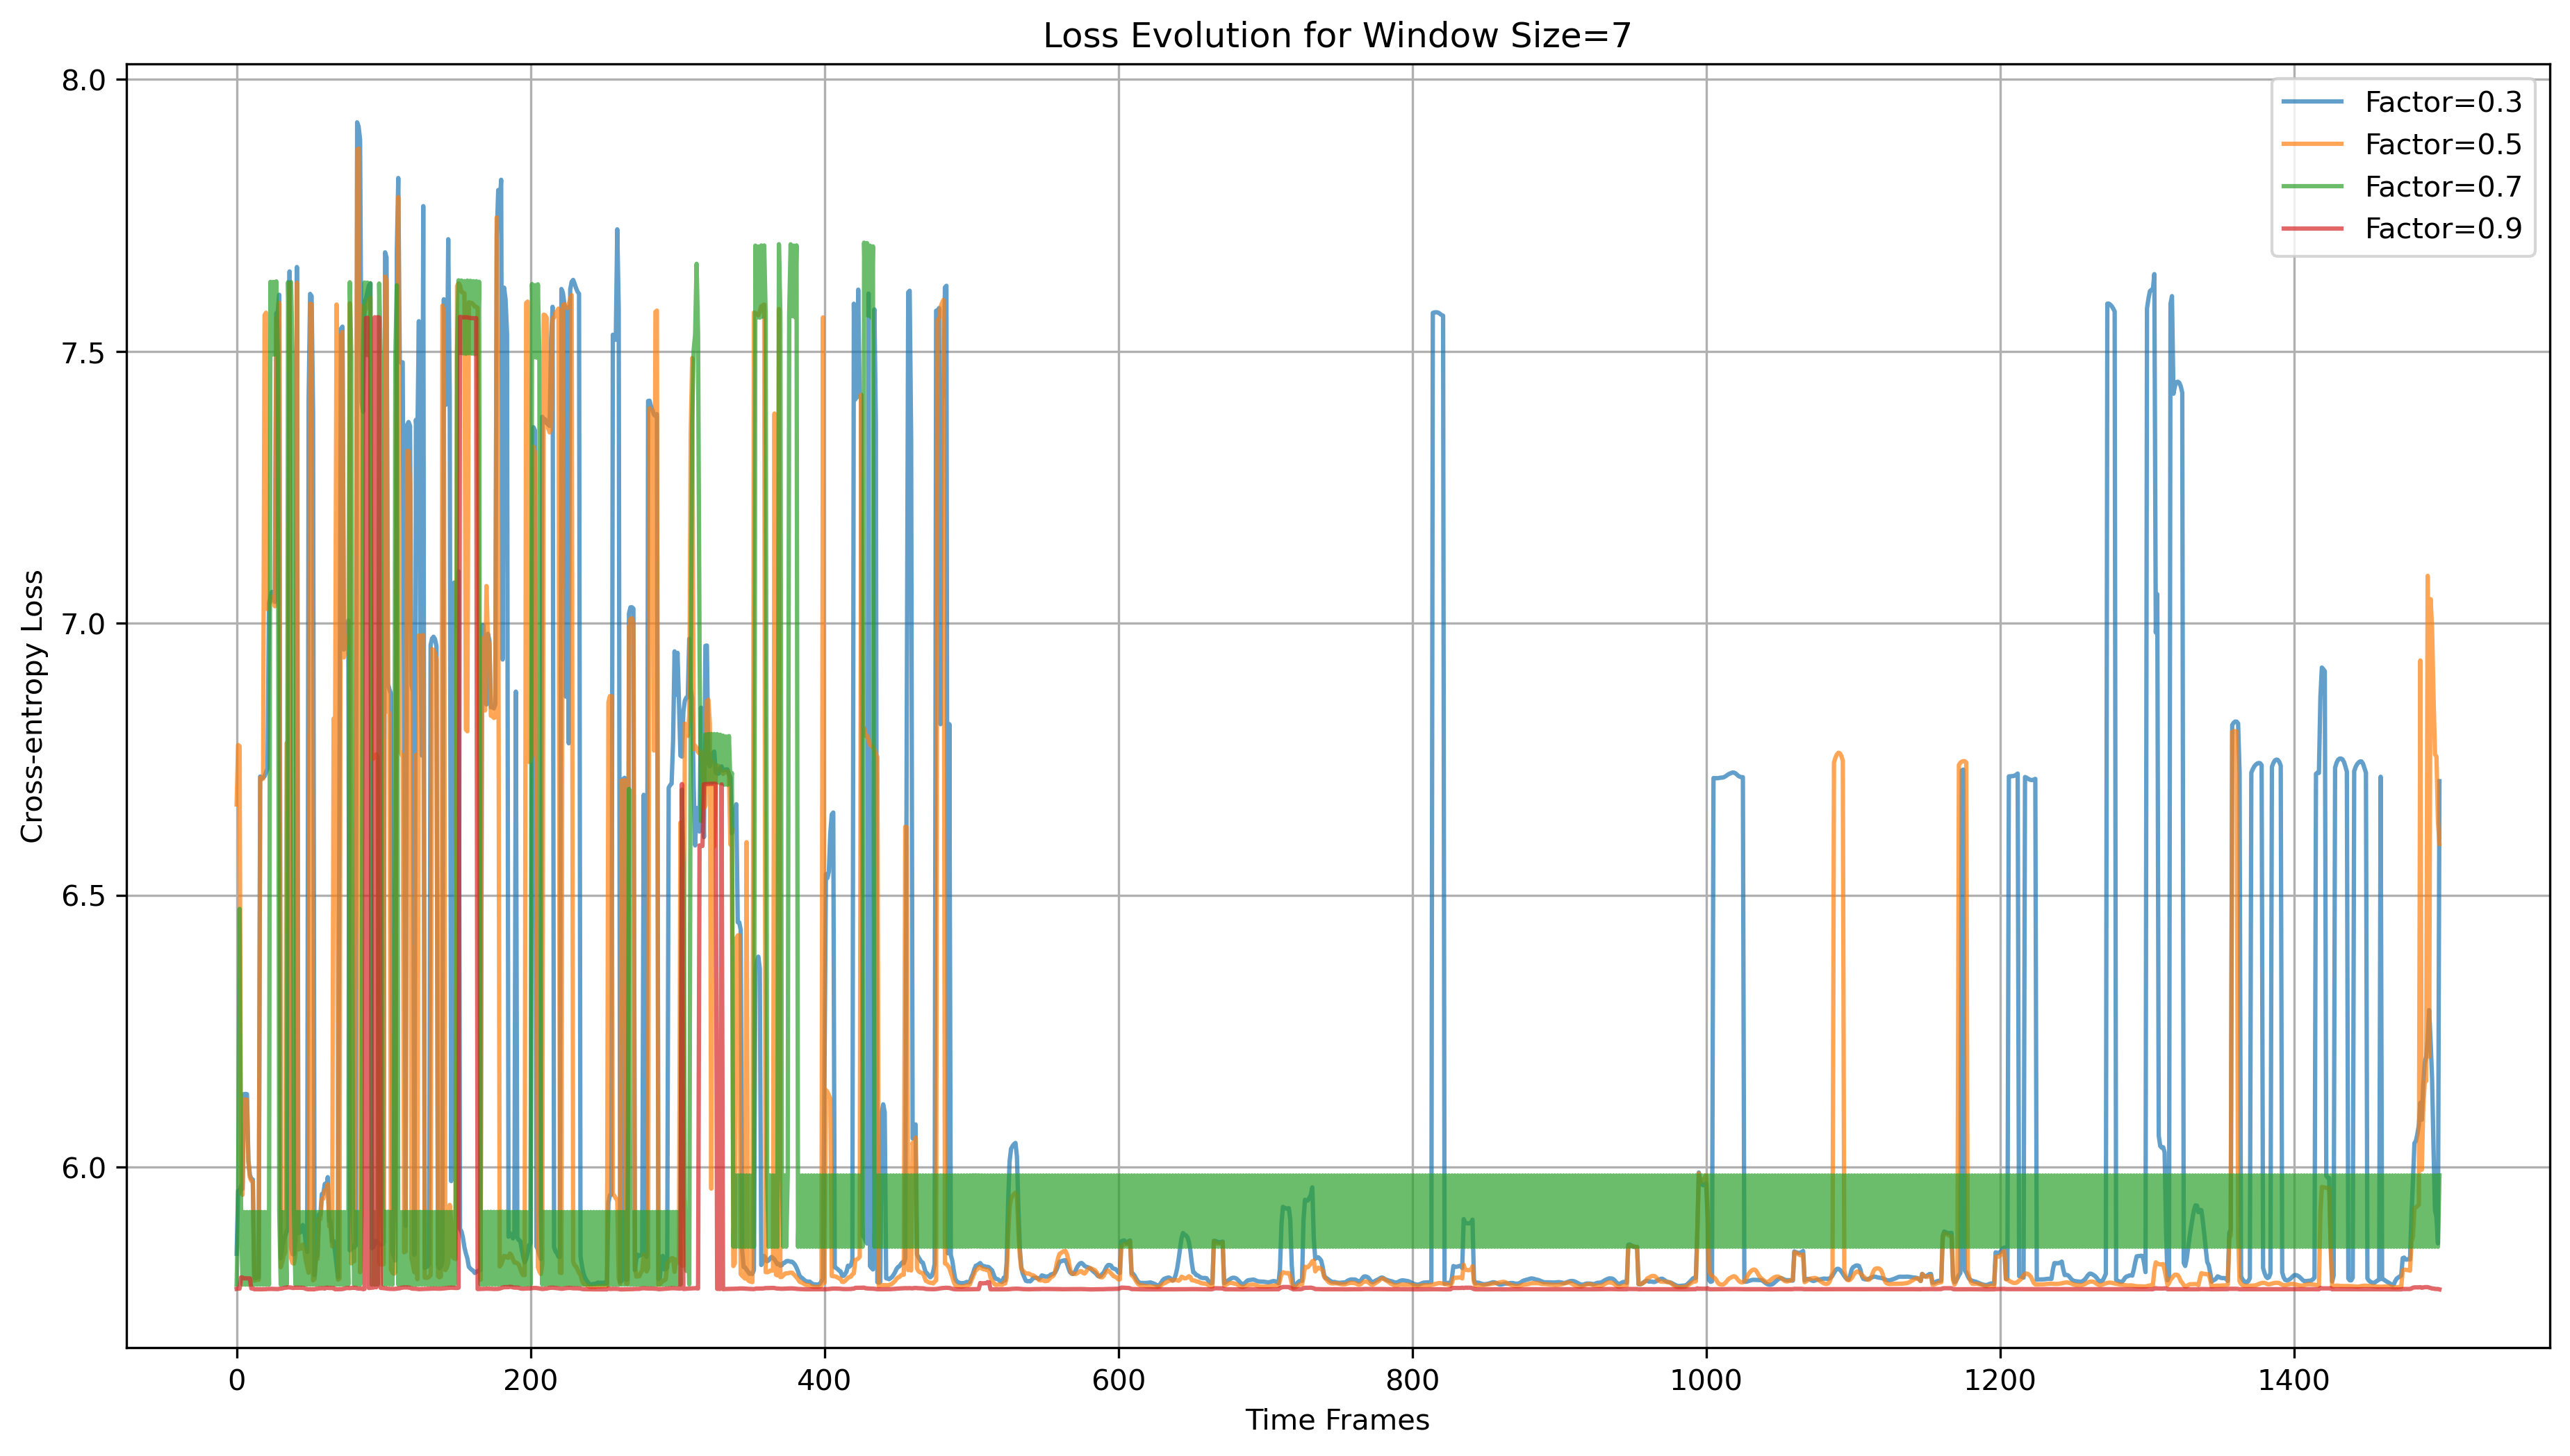
\includegraphics[width=0.48\textwidth]{figures/seq_len_7_comparison.png}
        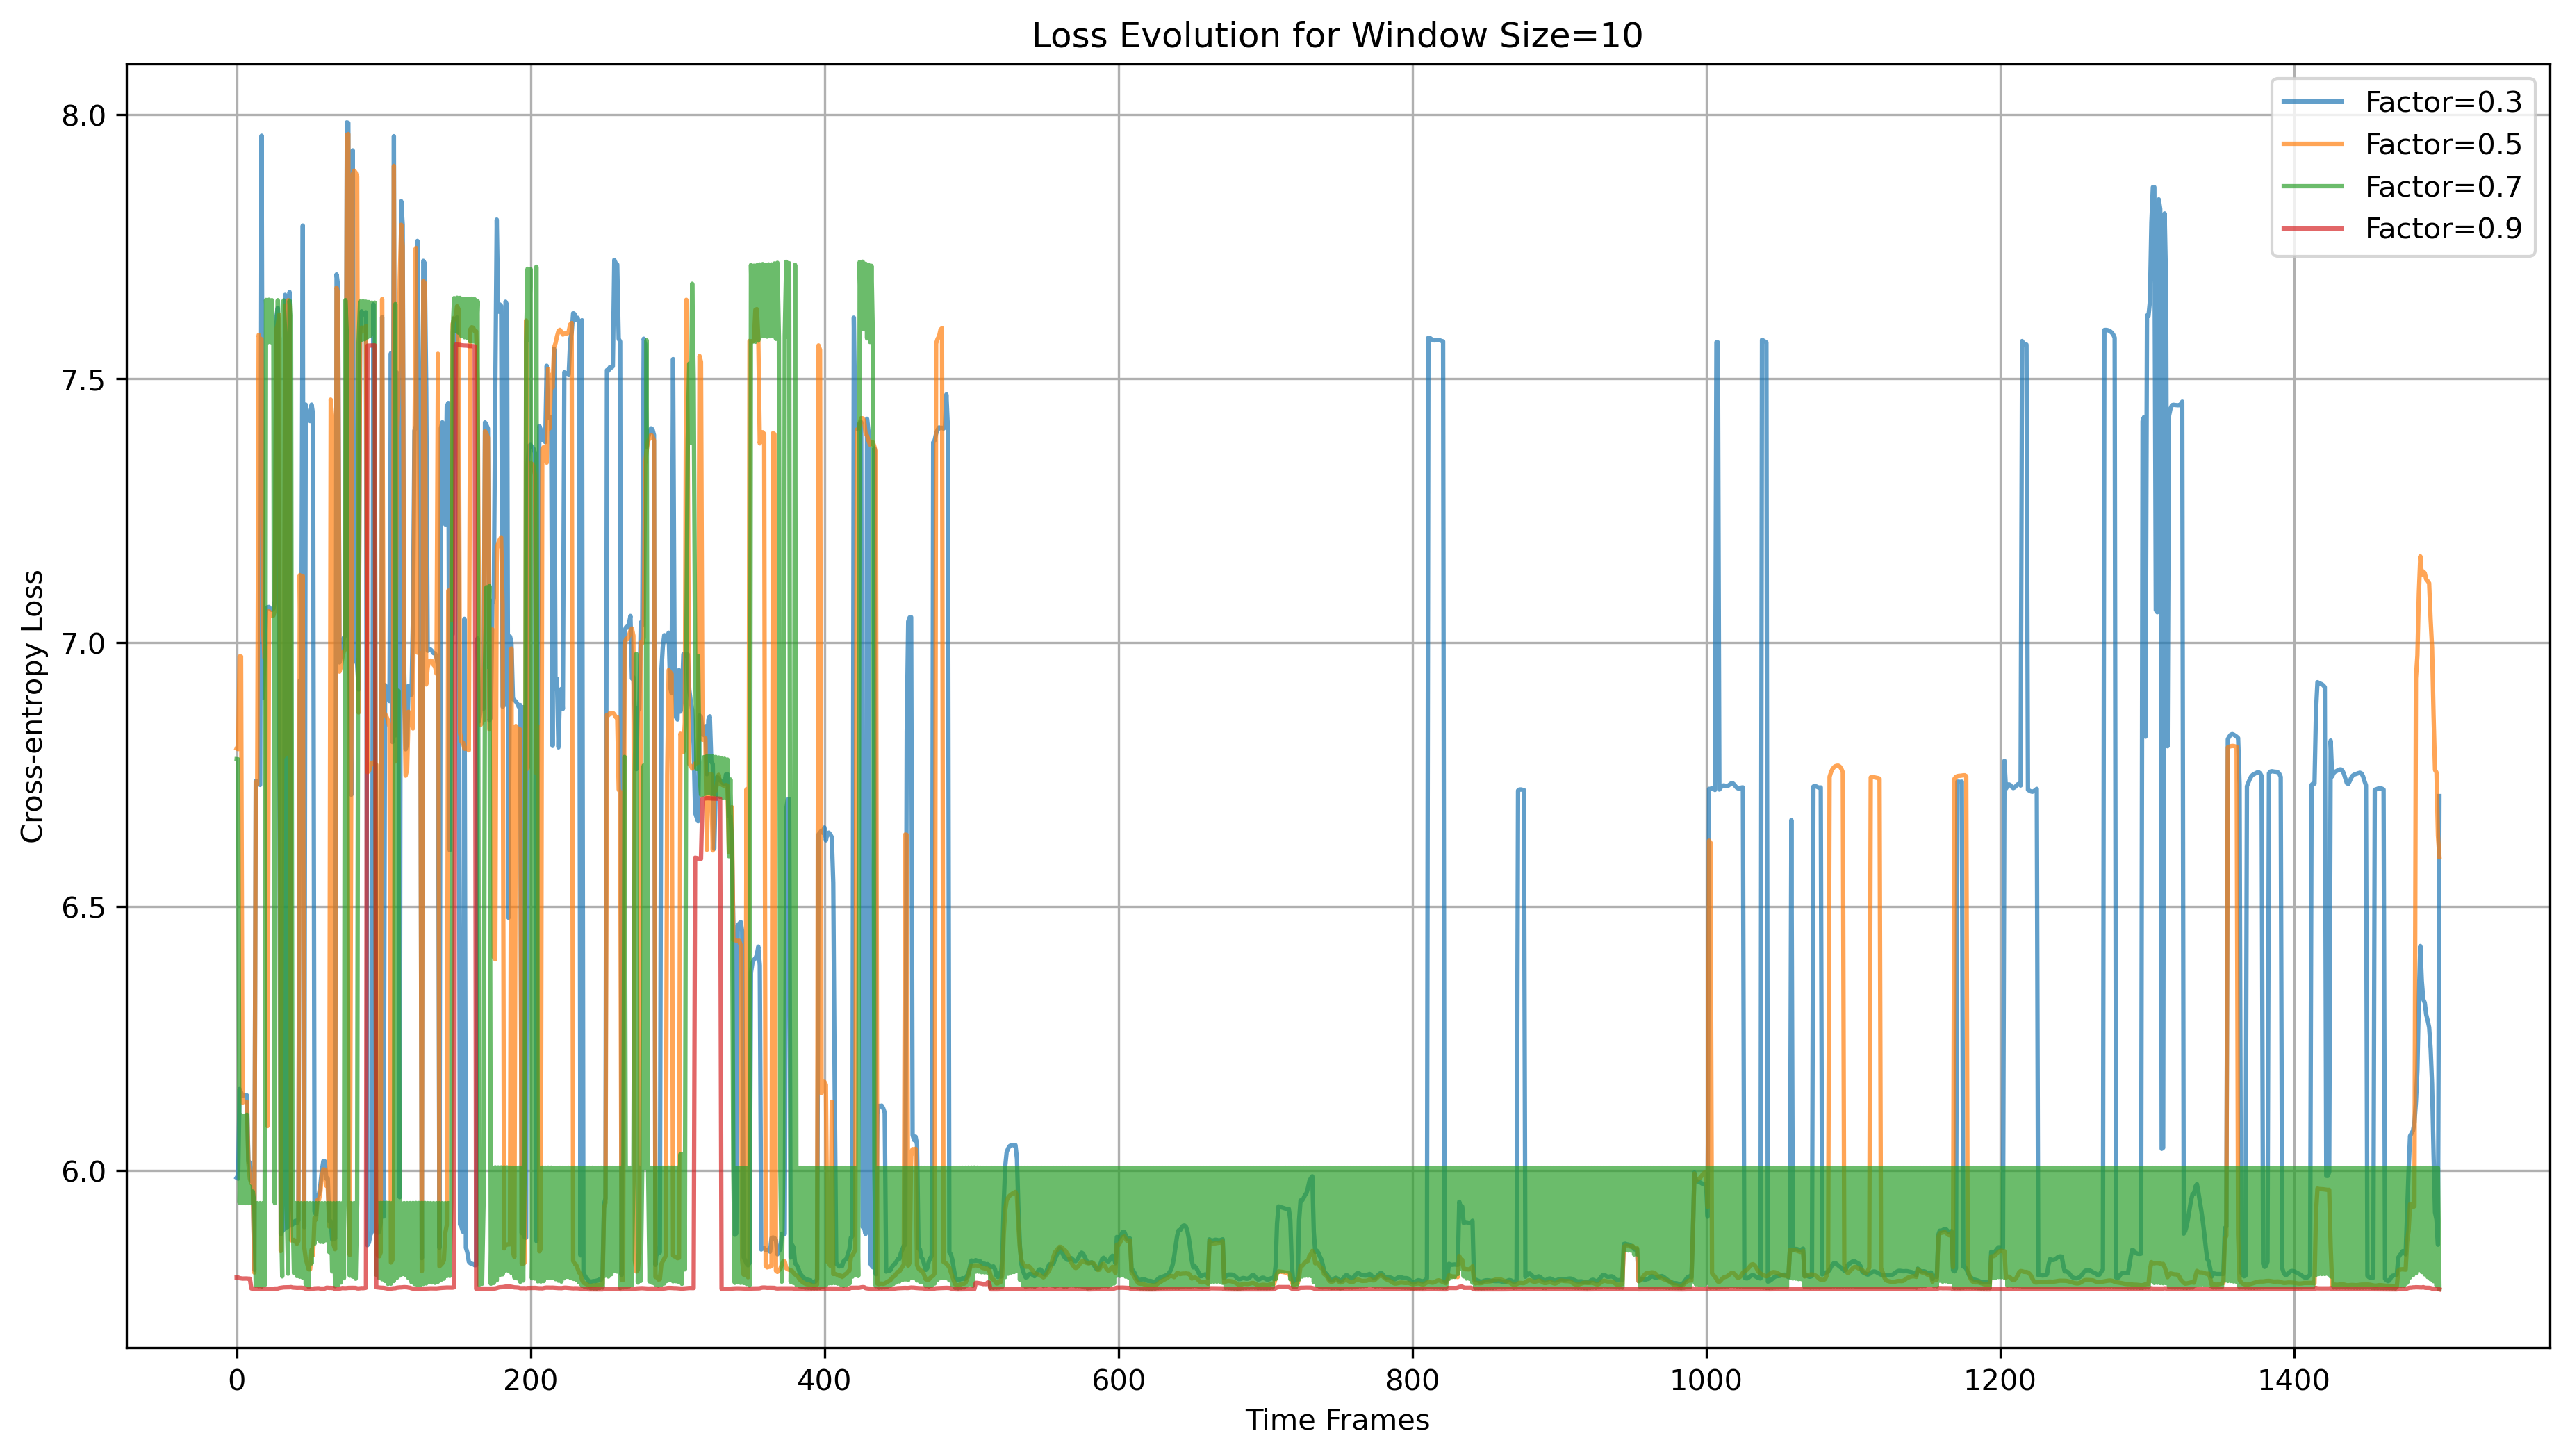
\includegraphics[width=0.48\textwidth]{figures/seq_len_10_comparison.png}
        
        \caption{Cross entropy loss over time frames for different suppression factors for a particular window size.}
        \label{fig:sequence_plots}
    \end{figure}


\end{document}
